% Based on template by MR

\documentclass[12pt,twoside,notitlepage]{report}

\usepackage{a4}
\usepackage{verbatim}
\usepackage{natbib}
\usepackage{graphicx}
\usepackage{listings}
\usepackage{bm}
\usepackage{amssymb}
\usepackage{subfigure}
\usepackage{algorithm2e}
\usepackage{color}

\definecolor{dkgreen}{rgb}{0,0.6,0}
\definecolor{gray}{rgb}{0.5,0.5,0.5}
\definecolor{mauve}{rgb}{0.58,0,0.82}

\lstset{frame=tb,
  language=Python,
  aboveskip=3mm,
  belowskip=3mm,
  showstringspaces=false,
  columns=flexible,
  basicstyle={\small\ttfamily},
  numbers=none,
  numberstyle=\tiny\color{gray},
  keywordstyle=\color{blue},
  commentstyle=\color{dkgreen},
  stringstyle=\color{mauve},
  breaklines=true,
  breakatwhitespace=true
  tabsize=3
}

\input{epsf}                            % to allow postscript inclusions

\raggedbottom                           % try to avoid widows and orphans
\sloppy
\clubpenalty1000%
\widowpenalty1000%

\addtolength{\oddsidemargin}{6mm}       % adjust margins
\addtolength{\evensidemargin}{-8mm}

\renewcommand{\baselinestretch}{1.1}    % adjust line spacing to make
                                        % more readable

% Resize over-large graphics ( http://tex.stackexchange.com/questions/27083/can-i-conditionally-scale-an-image-with-graphicx )
\newcommand{\lwincludegraphics}[2][]{%
  \sbox{0}{\includegraphics[#1]{#2}}%
  \ifdim\wd0>\linewidth
    \resizebox{\linewidth}{!}{\box0 }%
  \else
    \leavevmode\box0
  \fi}

\newcommand{\msg}[1] {{\bf #1}}         % \msg command for formatting Paxos messages
\newcommand{\op}[1]  {{\bf #1}}         % \op  command for formatting database operations
\newcommand{\superscript}[1]{\ensuremath{^{\textrm{#1}}}}
\newcommand{\subscript}[1]{\ensuremath{_{\textrm{#1}}}}
\newenvironment{myquote}{\list{}{\leftmargin=0.3in\rightmargin=0.3in}\item[]}{\endlist}


\begin{document}

\bibliographystyle{unsrt}


%%%%%%%%%%%%%%%%%%%%%%%%%%%%%%%%%%%%%%%%%%%%%%%%%%%%%%%%%%%%%%%%%%%%%%%%
% Title


\pagestyle{empty}

\hfill{\LARGE \bf Charlie Shepherd}

\vspace*{60mm}
\begin{center}
\Huge
{\bf PDB: A Distributed Database Based on Paxos} \\
\vspace*{5mm}
Computer Science Tripos \\
\vspace*{5mm}
Churchill College \\
\vspace*{5mm}
\today  % today's date
\end{center}

\cleardoublepage

%%%%%%%%%%%%%%%%%%%%%%%%%%%%%%%%%%%%%%%%%%%%%%%%%%%%%%%%%%%%%%%%%%%%%%%%%%%%%%
% Proforma, table of contents and list of figures

\setcounter{page}{1}
\pagenumbering{roman}
\pagestyle{plain}

\chapter*{Proforma}

{\large
\begin{tabular}{ll}
Name:               & \bf Charlie Shepherd                        \\
College:            & \bf Churchill College                     \\
Project Title:      & \bf PDB: A Distributed Database Based on Paxos \\
Examination:        & \bf Computer Science Tripos, July 2013        \\
Word Count:         & \bf 11717 \\
Project Originator: & Charlie Shepherd                    \\
Supervisor:         & Stephen Cross                    \\
\end{tabular}
}


\section*{Original Aims of the Project}

\subsection*{Project aims}

I aim to implement a distributed database. This will be based on the Paxos protocol.

\subsubsection*{Paxos}

The first half of the project is to implement the Paxos protocol. This will be done in a module,
providing an interface which the database can then use to

The project must correctly implement the Paxos protocol.  The library must be capable of forming a
running network, in particular dynamic leader election, as well as achieving consensus on a
key/value store across the network.

The database must implement a subset of SQL, specifically. The database must have all ACID
properties, that is.

\section*{Work Completed}

All that has been completed appears in this dissertation.

\section*{Special Difficulties}

None.

\newpage
\section*{Declaration}

I, Charlie Shepherd of Churchill College, being a candidate for Part II of the Computer Science
Tripos, hereby declare that this dissertation and the work described in it are my own work,
unaided except as may be specified below, and that the dissertation does not contain material that
has already been used to any substantial extent for a comparable purpose.

\bigskip
\leftline{Signed: }

\medskip
\leftline{Date: \today}

\cleardoublepage

\tableofcontents

\listoffigures

\newpage
\section*{Acknowledgements}

I would like to thank my supervisor Stephen Cross for his invaluable assistance, this project
could not have been successful without him. \\
My DoS, Dr John Fawcett, for his help and support over the last three years. \\
Ed and Nick for their help. \\
Talal, Lizzie and Joe for always lending a friendly ear.

%%%%%%%%%%%%%%%%%%%%%%%%%%%%%%%%%%%%%%%%%%%%%%%%%%%%%%%%%%%%%%%%%%%%%%%
% now for the chapters

\cleardoublepage        % just to make sure before the page numbering
                        % is changed

\setcounter{page}{1}
\pagenumbering{arabic}
\pagestyle{headings}

\chapter{Introduction}

\section{Motivation}

\begin{myquote}
``... all working protocols for asynchronous consensus we have so far encountered have Paxos at their
core ...'' \\
Mike Burrows \cite{burrows06}
\end{myquote}

Consensus in a distributed system is a difficult problem. Multiple protocols have been
developed as a solution but one of the most important is the Paxos protocol.

Paxos was developed by Leslie Lamport and first described in his paper \emph{The Part Time
Parliament} \cite{lamport98}.  The paper was first submitted for review in 1990 but its style,
which portrayed the protocol as a physical voting system in Ancient Greece, meant that it was not
published in a journal for a further eight years.

Lamport tried to disprove the existence of a protocol with the safety properties Paxos provides.
Instead, he ended up developing Paxos. Despite his assertion in \emph{Paxos Made Simple}
\cite{lamport01}, it has a reputation for being hard to implement.  With this in mind, I set out
to build a distributed database based on the protocol.  I took on the challenge of not only
implementing it, but also designing and coding a database layer on top. I wanted this database to
be functional, and have the properties expected of a standard database solution. This includes
SQL, transactions and ACID properties.

\section{Distributed Consensus Problem}

Consensus is an integral problem in distributed systems. The consensus problem is that of getting
all nodes in a distributed system to agree on a value. Formally, an algorithm that satisfies the
consensus problem satisfies three properties:

\begin{enumerate}
\item Agreement - all nodes must decide the same value.
\item Validity - the value that is decided upon must have been proposed by some node in the
	network.
\item Termination - all nodes eventually decide on a value.
\end{enumerate}

Decision is defined as follows - a process must decide on a value only once, and cannot change the
value once it has been decided.

\subsection*{Failure Modes}

Distributed networks must be able to deal with failure in a number of forms. Nodes may fail and
stop executing completely, this is known as the \emph{fail-stop} model. In practice, a more accurate
model is the \emph{fail-recover} model. This is where a node stops executing, then resumes execution
at a later time. This more accurately models real life, where asynchronous networks mean that it
may take an arbitrarily long time to receive a message, and that messages may arrive out of order
or not at all. The most general failure model is that of \emph{Byzantine failure}, where nodes may
respond incorrectly or even deliberately lie in order to mislead the protocol. In practice this is
unlikely, and can be mediated using checksums, message digests and authentication. In the
Preparation chapter I will go into detail about the types of failure that my database can handle.

\subsection*{2 Phase Commit}

2 Phase Commit is one of the simplest protocols that solves the Distributed Consensus problem. The
co-ordinator asks each node in the cohort to commit the value it suggests\footnote{i.e. this is
a binary decision, commit or abort. If a node wants a different value it must initiate its own
round of 2PC.}. If all nodes agree then it sends a message telling each member to commit, otherwise
it sends a message to each member telling them to abort. This is very efficient, with a message
cost of $3n$ for a network of $n$ nodes.

However, the problem with the 2PC protocol is its lack of tolerance to failures. Consider if the
co-ordinator fails during the protocol: some nodes in the cohort will have received a message from
the co-ordinator and voted and some may not. The nodes that have voted may be blocked, having
taken out locks when they voted commit. In order to proceed, the protocol can fall back to a
recovery node, which tries to complete the protocol by messaging all the nodes and gathering their
responses, then making a decision to commit or abort and finishing the protocol by informing all
nodes of the decision. However, if during that recovery, a member of the cohort crashes then
recovery becomes impossible, as the recovery node cannot recreate the state of the network and
therefore cannot make a decision to commit or abort.

\subsection*{3 Phase Commit}

3 Phase Commit is a modification to 2 Phase Commit that solves this problem by splitting the commit
phase into two, the pre-commit phase and the finalise phase.

As nodes only transition from one phase to the next when every node has replied to the previous
message, the case where it is not possible for one node to commit but another has already
committed the transaction cannot occur. If a node cannot commit, the furthest any other node in
the network can proceed is the pre-commit phase, while if a node has already committed then other
nodes must have at least reached the pre-commit phase.

This means if the co-ordinator crashes, the recovery node can reconstruct the state of the
transaction by querying any node in the
cohort. If that node is in the pre-commit phase, then every node must have voted commit and it is
safe to finish the protocol by telling all nodes to commit. If the node is not yet in the pre-commit
phase, then the operation has not been committed and it is safe to abort or restart the
transaction.

3PC still suffers from a flaw, however, in that it cannot recover from network partition. If the
network is partitioned such that all nodes in the cohort that are the pre-commit phase are on one
side of the partition and all nodes that are not are on the other side, then the first side of the
partition will complete the recovery and the other side will abort the operation, leaving the
network in an inconsistent state when the partition is resolved.

\subsection*{Paxos}

% http://betathoughts.blogspot.co.uk/2007/06/brief-history-of-consensus-2pc-and.html
% The kernel of Paxos is that given a fixed number of processes, any majority of
% them must have at least one process in common. For example given three
% processes A, B and C the possible majorities are: AB, AC, or BC. If a decision
% is made when one majority is present eg AB, then at any time in the future when
% another majority is available at least one of the processes can remember what
% the previous majority decided. If the majority is AB then both processes will
% remember, if AC is present then A will remember and if BC is present then B
% will remember.
%
% Paxos can tolerate lost messages, delayed messages, repeated messages, and
% messages delivered out of order. It will reach consensus if there is a single
% leader for long enough that the leader can talk to a majority of processes
% twice. Any process, including leaders, can fail and restart; in fact all
% processes can fail at the same time, the algorithm is still safe. There can be
% more than one leader at a time.
%
% Paxos is an asynchronous algorithm; there are no explicit timeouts. However, it
% only reaches consensus when the system is behaving in a synchronous way, ie
% messages are delivered in a bounded period of time; otherwise it is safe. There
% is a pathological case where Paxos will not reach consensus, in accordance to
% FLP, but this scenario is relatively easy to avoid in practice.

Paxos is a generalisation of 2PC and 3PC that handles more failure modes\cite{gray2006}. While 3PC
can handle failures, it only handles \emph{fail-stop} failures, not \emph{fail-recover} failures.
This is unfortunate, as computer networks are asynchronous networks, and can therefore be modelled
using a fail-recover model to account for arbitrary delays from messages being sent to being
received (fail-stop would mean messages can only be dropped, not delayed for an arbitrary length
of time).

Paxos relies on the fact that any majority of nodes in a network has at least one member in common
with any other majority. Therefore if the constraint that any decision must be made by a majority
of nodes is enforced then, once a decision is made, in any subsequent decision there will be at
least one member who was present in the previous decision. This is the central tenet of Paxos,
where a majority is known as a \emph{quorum}.

Brewer's CAP theorem\cite{brewer2000}\cite{gilbert2002} states that in the face of a
network partition, a distributed system can only provide availability or consistency, but not
both. A key advantage of Paxos is that it can guarantee consistency during a network partition.
This is in contrast to 3PC, which provides availability.

However, a potential drawback to this is that Paxos does sacrifice availability. This is in the
form of a pathological case where it will not make progress, i.e., there is no upper bound on the
time it will take to achieve consensus (it may never terminate). This is due to the FLP
impossibility proof \cite{fischer85}, which states that it is impossible to guarantee liveness in
an asynchronous network where there is at least one failure.  In practice it is a situation that
is relatively easy to avoid, and is not a serious concern.

\section{Databases}

\subsection*{ACID}

Commonly all databases provide ACID properties. ACID stands for:

\begin{itemize}
\item Atomic - an operation is either performed in its entirety or is not performed at all.
\item Consistent - the database remains in a \emph{consistent} state at all times, where being
	consistent is defined as being valid according to rules that ensure database integrity.
\item Isolated - one operation cannot see the intermediate state due to another operation occurring
	at the same time.
\item Durable - once an operation is `committed' it is permanently stored - the effects of it will
	not be lost.
\end{itemize}

There are many reasons why ACID is a key requirement of most databases. ACID makes it far easier
for application developers to reason about concurrency in a system where there may be multiple
clients reading and writing the same data simultaneously. It also enable effective abstraction, as
the atomicity requirement in particular gives the well defined characteristics when an operation
or transaction fails. ACID also provides clear guarantees with regard to data stability and
longevity, in particular how this relates to consistency, so that users can be clear as to the
overall state of the system.

\subsection*{Comparison between centralisation and distributed databases}

Databases are generally found in either centralised or distributed topologies. A centralised
database is a single node in a single location. In general, centralised databases are simpler in
design and also generally simpler to organise, edit, query and to backup. It is
easier to maintain the integrity of data on a centralised database, as there is only one
`current' version of the data under consideration.

In contrast, distributed databases are more resilient and scalable than centralised databases.
There is no longer a single point of failure, and they can be extended by adding nodes, although
this will have a point of diminishing returns. Distributed databases are often more complex in
design, as a distributed database is a generalisation of centralised one.

\subsection*{Existing Paxos databases}

Paxos has recently become a very popular algorithm for ensuring distributed consensus. One good
example is Google using it for `Chubby', their distributed lock service described in both
\emph{The Chubby lock service for loosely-coupled distributed systems}\cite{burrows06} and
\emph{Paxos Made Live}\cite{chandra07}. This underpins their BigTable distributed database which
is used across Google.

\emph{Paxos Made Live}\cite{chandra07} says ``While Paxos can be described with a page of
pseudo-code, our complete implementation contains several thousand lines of C++ code'', which
gives an indication of how intricate implementing Paxos actually is.  The paper described the
difficulty of producing a production-ready system in practice, and how moving from a theoretical
perspective to a practical one presented several problems. These included an imprecise
specification of the system and several real world faults that Paxos cannot deal with.

% \emph{Paxos Made Moderately Complex}\cite{renesse11} is another paper describing an implementation
% of Paxos by Robbert van Renesse at Cornell University.

\cleardoublepage

\chapter{Preparation}

\section{Requirements Analysis}

Given the brief to design and create a protocol and a database there is a huge amount of scope for
variety in the project. Requirements Analysis narrows down the purpose of a project to formal
goals which can easily be objectively verified against the finished project.

\subsection*{Paxos}
\paragraph{Correctness} Above all, the implementation of Paxos must be correct. This means that it
must conform to the description of the algorithm specified in \emph{The Part Time Parliament}
\cite{lamport98}.
\paragraph{Dynamic node membership} The implementation of Paxos must be able to support nodes
joining and leaving dynamically without losing correctness.

\subsection*{Database}
\paragraph{Encapsulation} The database must be a separate module to Paxos, and must be layered on
top of the API provided by the Paxos module.
\paragraph{Distributed} The database must be distributed. Any node in the network must have the
same capabilities as any other node in the network.
% homogenous
\paragraph{Transactions} The database must support transactions, that is, composite groups of operations.
\paragraph{ACID} The database must provide ACID properties through these transactions. ACID
properties are Atomicity, Consistency, Isolation and Durability. This means transactions can be
aborted, returning the database to the state before the transaction was started. Transactions must
also operate in isolation with each other.
\paragraph{SQL} The interface to the database must be SQL. It may be a limited form of SQL, as the
main priority of the project is the protocol and database design, rather than the interface.

\section{Software Engineering}

In order for the project to be a success, clear software engineering practices must be followed.

\subsection{Development Technique}

There are a number of techniques for developing software. The classic software development
strategy is the Waterfall model. This follows the steps of Requirements and Specification, Design,
Implementation, Verification and Maintenance. I decided against using this and instead using the
Spiral Model. The Spiral Model uses the steps of the Waterfall model but repeats them several
times, iteratively working towards the final result.

The Spiral Model is more suitable for my project because although I have set out my formal
requirements, there is still a lot of uncertainty in the project. I have not designed a network
protocol or a database before and I have not implemented Paxos before. This means that it is
likely I will encounter unexpected difficulties in developing my project that may lead me to
change or shift my requirements. The Spiral Model is more flexible than the Waterfall Model in
this case.

\subsection{Language Choice}

There are many languages this project could be implemented in, but the two main choices were the
two languages I have the most experience in: C and Python. They are reasonably different languages
--- C is a compiled low-level language, while Python is an interpreted high level language.

I decided to use Python for a variety of reasons:
\begin{itemize}
\item Python handles memory allocation internally, whereas whilst C provides great precision over memory
allocations, it also allows much more potential for memory handling errors.
\item Python is more concise than C and as a higher level language should allow me to develop several
prototypes without being impeded by focusing on details early on.
\end{itemize}

Also as my project is a network application, it should be mainly IO bound rather than CPU bound.
This means that the speed of the implementation language should not be a concern, as the speed
limitations of the implementation are unlikely to affect the performance of the project compared
to the limitations of the network.

\subsection{Module Dependencies}

Twisted is a Python framework used for event driven network programming. It contains support for
many different protocols, making writing efficient networking code a lot easier.  It is single
threaded, which means I will not have to worry about concurrency issues in my project. Twisted is
licensed under the MIT license so there are no license issues in using it for my project.

The other module I decided to use is PyParsing, a Python module for programmatically creating a
parser in Python. I decided to use this for parsing input SQL, as it will make the task
substantially simpler. I have already used PyParsing briefly, so I have a small amount of
familiarity with it. PyParsing is also distributed under the MIT license.

\subsection{Version Control and Backup}

Version control is a necessity in any software project. I decided to use a decentralised version
control system (DVCS) for a number of reasons. DVCSs have a distributed structure rather than
using a central or master server. This makes it possible to commit changes locally without needing
a connection to any server. DVCSs also have advanced branching and merging tools, making it easier
to branch to develop experimental features, and then merge the feature in later.

Another advantage is being able to `push' the repository to any number of remote locations, as
an online copy or backup. I will use this as my backup strategy, keeping everything related to
my project in my repository and pushing every few hours to two different servers.

While most DVCSs are very similar, I chose Git as it is the version control system I have the most
familiarity with.

\subsection{Testing}

In order to ensure I can have confidence that my project works correctly I will need to write
tests. I will write unit tests for the main modules of my project, both for expected input and
also that it handles bad and malformed input correctly and as expected. Tests are also useful for
expressing the API usage of the different modules of the project and checking that the interfaces
connect sensibly. I will perform regression testing, that is, every time there I fix a bug I will
add a test ensuring any regression causing the bug again will make the test fail.

I will run tests every time I make a commit, as they are quick to run and confirm that the project
is working correctly. Twisted has a unit testing framework that I will use as it easily
facilitates testing asynchronous programs, something that would be harder in other unit testing
frameworks available in Python.

\section{ACID}

ACID is an acronym for a set of properties that nearly all databases provide. These properties
provide certain guarantees about how the database handles transactions so that programmers using
the database can be confident that their transactions will be processed reliably. Here I will go
into some detail about what each of these properties mean.

\subsection*{Atomic}

Atomicity means that either an operation completes or it does not, there is no `halfway' state.
This means that the programmer using the database does not need to worry about cleaning up after
an operation, because if it does not succeed they can simply retry it without needing to worry about
the state it has left the database in. Atomicity also applies to transactions in the same way ---
When a transaction, composed of smaller single operations (for example, INCR
B, READ A $\rightarrow$ X, WRITE X + 10 $\rightarrow$ A), is executing, it would be indesirable
for some of the operations to complete and some not to. In this example, if the database has the
invariant $A = 10\times B$ and B was incremented but then the transaction failed before A was
updated, the database would be left in an invalid state.

\subsection*{Consistent}

Consistency is very closely related to atomicity, as consistency refers to a property of the
database, and atomicity refers to a property of operations performed on the database. In the
example used for atomicity, the database had the constraint that $A = 10\times B$. Operations and
transactions should transform the database from one consistent state to another. This becomes more
pertinent in distributed databases, as operations may be received in one order at one node and in
a different order at another node. If they are applied in the order that they were received then
the two nodes are likely to be in inconsistent states.

\subsection*{Isolated}

Isolation is the property that ensures that if one transaction is in the process of completing,
another transaction cannot see the intermediate state. Transactions should be processed as if they
were executed sequentially. It ensures that transactions that execute concurrently to each other
are also invisible to each other. This means a transaction should not be able to tell whether
another transaction is executing or not.

\subsection*{Durable}

The durable property refers to the permanence of a transaction. Once a database reports that a
transaction has been committed, it should persist in the database even in the face of power loss or
crashes. This is typically achieved by using a write-ahead log that is append only, so that in the
event of a crash, the database can reconstruct the state of all transactions reported as
`committed'. Distributed systems have an added complication of co-ordinating this property
across the network before the transaction can be reported as `committed'.

\section{Distributed Consensus Protocols}

\subsection*{2 Phase Commit}

\begin{figure}[htb]
\centering
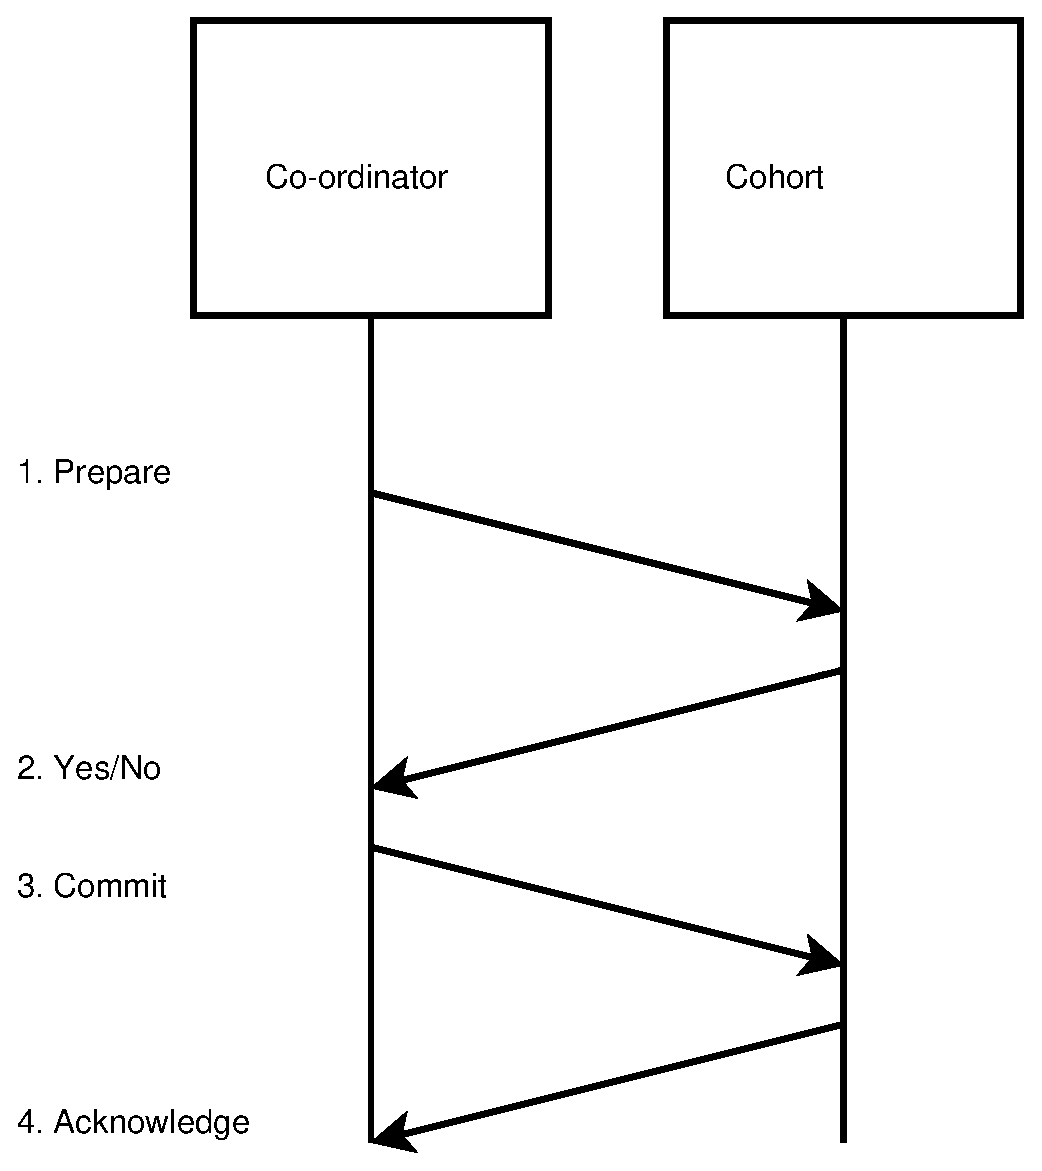
\includegraphics[scale=0.5]{figs/two-pc.eps}
\caption{\label{fig:two-pc}Two Phase Commit}
\end{figure}

2 Phase Commit (2PC) is one of the simplest consensus protocol, and one of the most brittle. The
basic message flow is shown in figure~\ref{fig:two-pc}. It has two phases:

\begin{enumerate}
\item The co-ordinator (the node initiating the protocol) sends a \msg{PROPOSE} message to each
	node in a cohort of size $N$, asking them to accept the value proposed.
\item The nodes reply with a \msg{YES} or \msg{NO} reply.
\item If all nodes respond with a \msg{YES} message, the co-ordinator sends a \msg{CONFIRM} message. Otherwise, if
	any node responds with a \msg{NO} message, it sends an \msg{ABORT} message to all nodes.
\item Nodes reply with an \msg{ACK} message, and the co-ordinator marks the transaction as
	complete when all nodes have acknowledged it.
\end{enumerate}

% S comment: split into 2 paragraphs and use footnotes

2PC solves the consensus problem in a failure free network. However the protocol can suffer from a
number of limitations if failures are allowed. If the co-ordinator crashes before sending
any messages, consensus is trivially satisfied. However, if the co-ordinator crashes after sending
$x$ messages, where $1 \le x < N$, the protocol cannot continue -- it is blocked on the
co-ordinator resuming, and if it never resumes then some members of the cohort are blocked
permanently. In fact, once a node has sent a \msg{YES} message, it is blocked until it receives a
response. This is a big disadvantage for a concurrent system. While there are extensions to
resolve the problem of a crashing co-ordinator, these do not fix the fundamental problem of using
a blocking protocol in an asynchronous network. \footnote{These extensions often involve a `watchdog' or
`recovery' node. This is still not a satisfactory solution as the simultaneous crash of the
co-ordinator and a cohort member means the state of the network is not recoverable (i.e., it is
not possible to tell if the cohort member who crashed voted \msg{YES} or \msg{NO}.)}

\subsection*{3 Phase Commit}

\begin{figure}[h!]
\centering
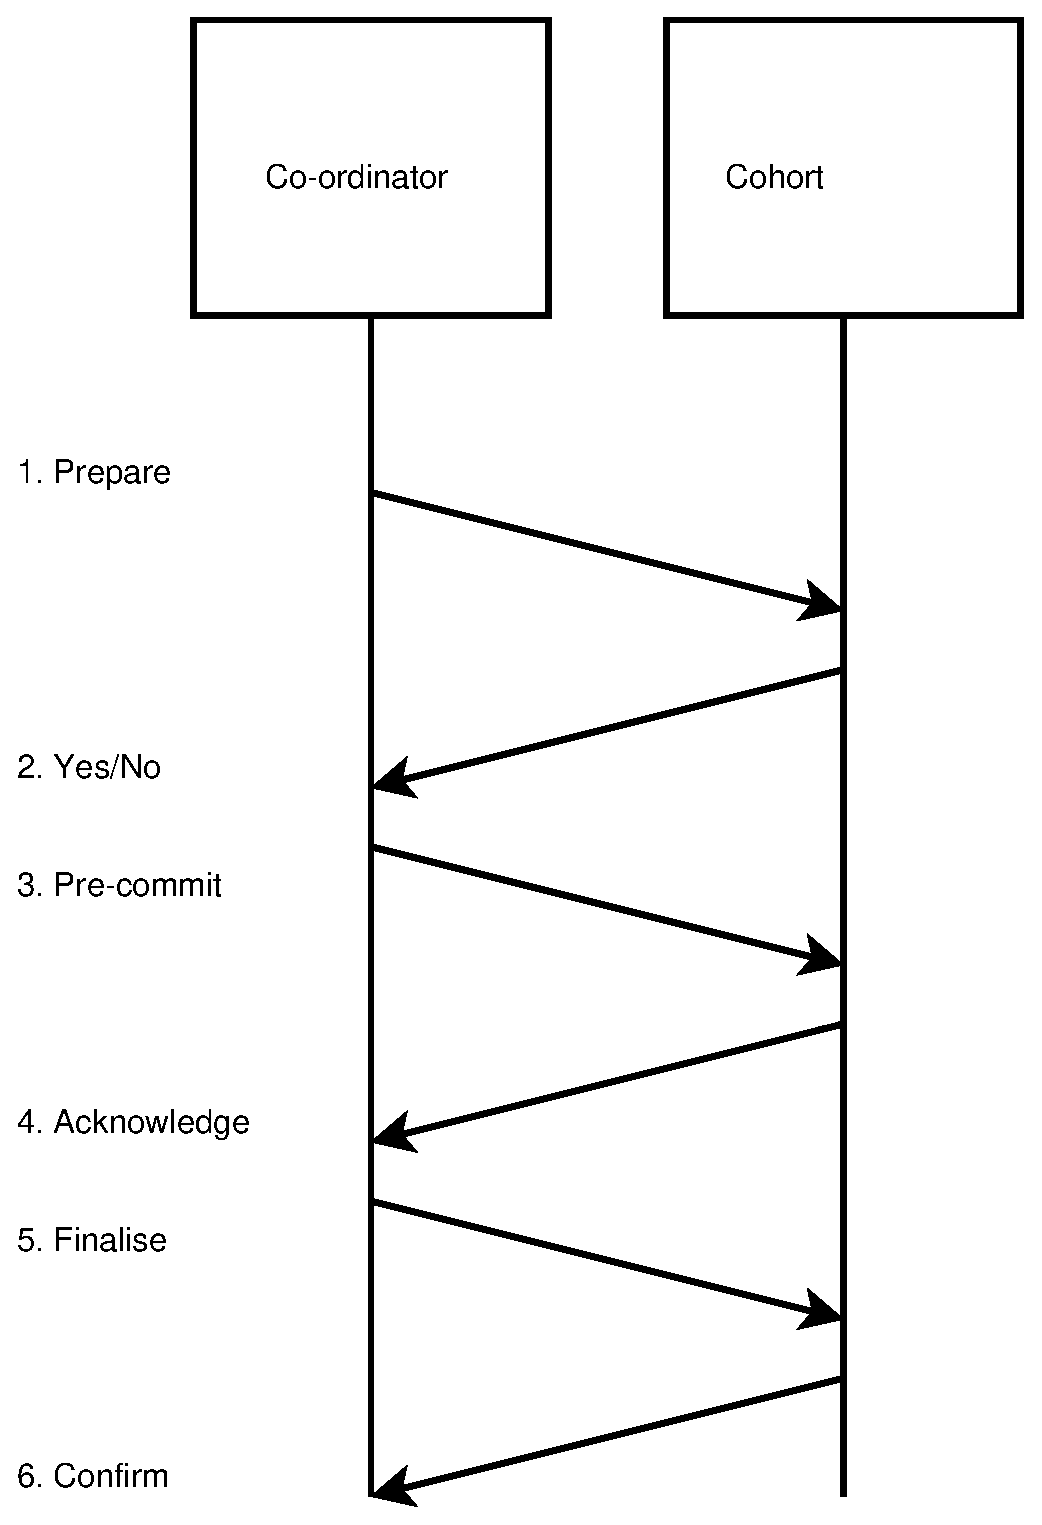
\includegraphics[scale=0.5]{figs/three-pc.eps}
\caption{\label{fig:three-pc}Three Phase Commit}
\end{figure}

3 Phase Commit (3PC) is a modification of 2PC that turns it from a synchronous protocol into an
asynchronous protocol. This is done by adding a third phase, so that timeouts can be used to assert
the state of the system at any point in time. Again the basic message flow is shown in
figure~\ref{fig:three-pc}. The three phases are:

\begin{enumerate}
\item \msg{Prepare}: the co-ordinator asks the cohort members if they can perform the operation. At
	this stage if there is a failure or timeout, the co-ordinator aborts the transaction.
\item The cohort respond with a \msg{YES} or \msg{NO}. Again, if there is a failure or timeout the cohort
	member considers the transaction aborted.
\item \msg{Pre-commit}: If the co-ordinator receives \msg{YES} messages from every member of the
	cohort, it sends a \msg{Pre-commit} message to them all, otherwise it aborts the
	transaction. It also aborts in the case of a failure or timeout.
\item \msg{Acknowledge}: If the cohort member receives a \msg{Pre-commit} message, it replies with
	an \msg{Acknowledge} message. If the co-ordinator aborts, or there is a failure or
	timeout, the cohort member aborts.
\item \msg{Finalise}: If the co-ordinator times out, it aborts the transaction. Otherwise, when it
	has received \msg{Acknowledge} messages from every cohort member it sends a \msg{Finalise}
	message to them all.
\item \msg{Confirm}: Once a cohort member has received a \msg{Finalise} message, it commits the
	transaction, even if the co-ordinator fails. It can reply with a \msg{Confirm} message.
\end{enumerate}

This fixes the problem of node failure, but still suffers from a significant problem. If there is
a network partition, and all nodes who voted \msg{YES} are in one half and all nodes who voted
\msg{NO} are in the other, both partitions will recover into different, inconsistent states.
Brewer's CAP theorem \cite{gilbert2002} says that consensus and availability cannot both be
achieved during a network partition --  only one. 3PC opts for availability, but for a distributed
database with ACID properties it is preferable to have consensus. Paxos guarantees consensus at
the cost of lack of availability in a network partition.

\section{Paxos}

\subsection{Introduction}

Paxos is a distributed consensus algorithm. Paxos is failure tolerant for up to $F$
simultaneous failures in a network of $2F + 1$ nodes.

Paxos is actually a family of protocols, based around the same main algorithm. The Paxos algorithm
is an algorithm for agreeing on a single value across a network of processors. Paxos has several
safety and liveness properties:

\paragraph{Safety Guarantees}

\begin{itemize}
\item Integrity - every correct process decides at most one value, and if it decides some value
	$v$, then $v$ must have been proposed by some process.
\item Agreement - Every correct process must agree on the same value.
\item Non-triviality - Only a value that has been proposed can be chosen.
\end{itemize}

% Consistency
%     At most one value can be learned (i.e., two different learners cannot learn different values).[8][9]
% Only a single value is chosen
%
% Liveness(C;L)
%     If value C has been proposed, then eventually learner L will learn some value (if sufficient processors remain non-faulty).[9]
%
%
% A process never learns that a value has been chosen unless it has been

\paragraph{Liveness Properties}

\begin{itemize}
\item Some proposed value is eventually chosen
\item If a value is chosen, a process eventually learns it
\item Termination - Every correct process decides some value.
\end{itemize}

Paxos can tolerate certain kinds of failures. These are: messages being lost, delayed, repeated or
delivered out of order. It is correct even with multiple leaders, and will reach consensus if
there is a single leader that talks to a majority of processes twice.

% Paxos can tolerate lost messages, delayed messages, repeated messages, and
% messages delivered out of order. It will reach consensus if there is a single
% leader for long enough that the leader can talk to a majority of processes
% twice. Any process, including leaders, can fail and restart; in fact all
% processes can fail at the same time, the algorithm is still safe. There can be
% more than one leader at a time.
%
% Paxos is an asynchronous algorithm; there are no explicit timeouts. However, it
% only reaches consensus when the system is behaving in a synchronous way, ie
% messages are delivered in a bounded period of time; otherwise it is safe. There
% is a pathological case where Paxos will not reach consensus, in accordance to
% FLP, but this scenario is relatively easy to avoid in practice.

However Paxos cannot tolerate `rogue' processes, that is, processes deliberately sending
malicious or incorrect messages. There is a variant of Paxos called \emph{Byzantine Paxos} which
can tolerate this, albeit at a failure tolerance of $F$ for $3F + 1$ nodes. I will not go into
this variant further in this dissertation.

\subsection{Definitions}

\subsubsection*{Proposals}

In an instance of Paxos, values that can be accepted are called \emph{proposals}. A proposal is a
2-tuple of the form ($n$, $v$), where $n$ is the unique proposal number and $v$ is the value
proposed.

\subsubsection*{Proposal Numbering}

One of the assumptions that Paxos makes is that every proposal has a unique proposal number. This
is necessary so that proposals have a \emph{total order}. A total order means that every proposal
can be compared to any other proposal. This is necessary in order to
find the maximum ordered proposal. The conventional way to achieve this is to define a proposal
number as a 2-tuple of (sequence number, node address). These can be compared lexicographically,
and as node addresses are unique, every proposal number will be unique. In practice I plan to use
UUIDs as node identifiers, in order to be confident of their uniqueness.


\subsubsection*{Messages}

Paxos utilises several message types:

\begin{itemize}
\item \msg{Prepare(n)}, asking the recipient to respond with a \msg{Promise} not to
	accept any proposals numbered less than $n$.
\item \msg{Promise(n, m, v)}, promising to only accept proposals numbered greater than or equal to
	$n$. $m$ refers to the number of the highest proposal previously accepted by the recipient and
	$v$ is the value of that proposal. If they are not included and the message is in the form
	\msg{Promise(n)}, it is assumed that the recipient has not accepted any proposals
		previously.
\item \msg{AcceptRequest(n, v)}, asking the recipient to accept the proposal ($n$, $v$).
\item \msg{AcceptNotify(n, v)}, notifying the recipient that the sender has accepted the proposal
	($n$, $v$).
\end{itemize}

\subsection{How it works}

\label{sec:how-paxos-works}

The central concept of Paxos is that of majority vote. A \emph{quorum} is defined as a majority of
nodes in the system.  Paxos requires a quorum of nodes to accept a proposal before the proposal is
considered `learnt' by the network. As any quorum of nodes must share at least one node with any
other quorum, if a proposal is accepted by a quorum $Q$ and learnt, any subsequent decision taken
must involve at least one node $q \in Q$.

Paxos is comprised of two stages. First, a quorum of nodes $Q$ are sent \msg{Prepare} messages to
prepare them to accept a proposal. They respond with the greatest proposal they have previously
accepted. It is this key step which ensures that Paxos enforces consistency. In the second step,
the co-ordinating node sends out a proposal for nodes to accept. However, the value of this
proposal must be the value of the greatest proposal previously accepted by a node in $Q$.

\subsubsection*{Formal description of the algorithm}
In \emph{Paxos Made Simple} \cite{lamport01}, the actions of a Paxos node are split into three
roles - Proposer, Acceptor and Learner. Explaining it in terms of these roles is simpler, however
in practice they are combined into one client.

\subsubsection*{Proposer}

\paragraph{Phase 1}

To start a round of Paxos, the Proposer $P$ sends out a \msg{Prepare(n)} message to the acceptors in
the network with a unique proposal number, $n$. This proposal number $n$ must
be higher than any proposal numbers $P$ has sent for this instance of Paxos.

\paragraph{Phase 2}

If the Proposer receives replies from a quorum of acceptors, $Q$,
to its \msg{Prepare(n)} message, it sends the message \msg{AcceptRequest(n, v)} to all
$q \in Q$, where $v$ is defined as follows. If the message set $M$ is defined as
\begin{displaymath}
M = \{(\eta, \nu)~|~\msg{Promise(n, \bm{\eta}, \bm{\nu})}~\textrm{received by}~P\}
\end{displaymath}
then $v$ is defined as
\begin{displaymath}
\exists~(\eta', v') \in M.~\forall~(\eta'', \nu'') \in M.~\eta' \ge \eta'' \\
\end{displaymath}
\begin{displaymath}
v = v'
\end{displaymath}
That is, if $\sqsupset$ is an ordering over \msg{Promise} messages such that
\begin{displaymath}
	\msg{Promise(n, \bm{\eta_1}, \bm{\nu_1})} \sqsupset \msg{Promise(n, \bm{\eta_2}, \bm{\nu_2})}
	\iff \eta_1 > \eta_2
\end{displaymath}
then informally, $v$ is the value of the maximum \msg{Promise(n, $\bm{\eta}$, $\bm{\nu}$)} received by
$P$.\footnote{
As this is all in response to $P$'s \msg{Prepare(n)} message, $n$ has the same value for
every \msg{Promise} message in this phase.}

\subsubsection*{Acceptor}

Acceptors need to store a few variables. An acceptor $A$ stores:
\begin{itemize}
\item $\rho$ - the greatest proposal number that $A$ has received in a \msg{Prepare} message and
	responded to with a \msg{Promise} message.
\item $\eta$ - the highest-numbered proposal $A$ has accepted (initialised to $0$).
\item $\nu$ - the value of proposal $\eta$ (initialised to \verb+null+).
\end{itemize}

\paragraph{Phase 1}

If an Acceptor $A$ receives a message \msg{Prepare(n)}, and $n > \rho$, then it replies with the
message \msg{Promise(n, $\bm{\eta}$, $\bm{\nu}$)} and sets $\rho$ to $n$. This means it will not
accept any proposals numbered less than $n$. If it has not accepted any proposals yet then $\eta$
and $\nu$ will still be set to their initial values.

\paragraph{Phase 2}

If an Acceptor receives a message \msg{AcceptRequest(n, v)}, if $n > \rho$ it accepts the
proposal, setting $\eta := n$ and $\nu := v$. It also notifies Learners in the network of its
decision by sending an \msg{AcceptNotify(n, v)} message to them.

\subsubsection*{Learner}

For each proposal number, Learners must store a set containing the GUIDs of all Acceptors who have
accepted that proposal. When a Learner receives a message \msg{AcceptNotify(n, v)} from an
Acceptor $A$, it must add $A$ to the set of Acceptors who have accepted proposal $n$. When this
set becomes a quorum (ie, the size of the set $S$ becomes greater than $\frac{N}{2}$, where $N$ is
the size of the network), the Learner can `learn' the $v$ as the value decided on for that
instance of Paxos. Because of the properties of Paxos, once a quorum of acceptors has accepted the
proposal ($n$, $v$), the value of that instance will never change.

\subsection*{Examples}

The behaviour of Paxos is perhaps best explained with a few examples of different situations.

\subsubsection*{Normal Behaviour}

\begin{figure}[h!]
\centering
\lwincludegraphics{figs/paxos-msg-flow-usual.eps}
\caption{\label{fig:paxos-usual}Paxos Message Flow: Usual Behaviour}
\end{figure}

Figure~\ref{fig:paxos-usual} shows the message flow for a
complete round of Paxos if there are no failures and everything proceeds as expected. In this
case, then the behaviour is reasonably straightforward to follow. There are four message delays
until the proposed value is learnt.

\begin{enumerate}
\item \msg{Prepare(n):} The Proposer sends a \msg{Prepare} message to the Acceptors.
\item \msg{Promise(n):} The Acceptors all promise to accept proposals numbered $\ge n$, as they
	have not seen any \msg{Prepare} requests yet and therefore trivially cannot have promised
	to accept a proposal higher than $n$.
\item \msg{AcceptRequest(n, v):} The Proposer sends a value $v$, with the proposal number $n$, to
	the Acceptors.
\item \msg{AcceptNotify(n, v):} The Acceptors have not made any promises preventing them from
	accepting $n$, so they accept $v$ as the value for the round of Paxos and notify the
	Learner.
\end{enumerate}

\subsubsection*{Acceptor Failure}

\begin{figure}[h!]
\centering
\lwincludegraphics{figs/paxos-msg-flow-one-acceptor-fail.eps}
\caption{\label{fig:paxos-acceptor-fail}Paxos Message Flow: Acceptor Failure}
\end{figure}

Figure~\ref{fig:paxos-acceptor-fail} shows the same
scenario, but with a single Acceptor failing. In this case there is still a quorum of Acceptors
available, so behaviour carries on as normal. There are still four message delays until the
proposed value is learnt.

\begin{enumerate}
\item \msg{Prepare(n):} The Proposer sends a \msg{Prepare} message to the Acceptors.
\item Failure: Acceptor 3 fails.
\item \msg{Promise(n):} Acceptors 1 and 2 still promise to accept the proposal, for the same
	reason as before.
\item \msg{AcceptRequest(n, v):} The quorum size is 2, so a quorum of acceptors has responded, and
	the Proposer can continue as normal.
\item \msg{AcceptNotify(n, v):} The Learner receives \msg{AcceptNotify} messages from a quorum of
	Acceptors, so also continues as normal, learning the value $v$.
\end{enumerate}

\subsubsection*{Partition}

\begin{figure}[h!]
\centering
\lwincludegraphics{figs/paxos-msg-flow-partition.eps}
\caption{\label{fig:paxos-partition}Paxos Message Flow: Partition}
\end{figure}

% This is to get this figure on the next full page, ie *before* the duelling section rather than
% on a random page after it...
\begin{figure}[p]
\centering
\lwincludegraphics{figs/paxos-msg-flow-duelling.eps}
\caption{\label{fig:paxos-duelling}Paxos Message Flow: Duelling Proposers}
\end{figure}

Figure~\ref{fig:paxos-partition} shows what happens in a
network partition. A second Proposer is able to continue the instance of Paxos, and no
inconsistencies are allowed to occur in the network, as the left half of the partition is unable
to make progress until the partition is resolved, at which point it can learn the decisions made
by the half of the partition that was able to make progress.

\begin{enumerate}
\item \msg{Prepare(1):} The Proposer sends a \msg{Prepare} message to the Acceptors, but is only
	able to successfully message one of them.
\item \msg{Prepare(2):} A second Proposer simultaneously sends a \msg{Prepare} message to the
	Acceptors, and is able to reach a quorum.
\item \msg{Promise(1):} The Acceptor on the left side of the split replies with a \msg{Promise},
	but does not make up a quorum.
\item The first Proposer times out. It could restart with a higher proposal number, but in this
	case it will be unable to make any progress until the partition is resolved.
\item \msg{Promise(2):} The Acceptors on the right side of the split both reply with a
	\msg{Promise}, making a quorum.
\item \msg{AcceptRequest(2, b):} The second Proposer asks the Acceptors to accept \verb+'b'+ as the
	value.
\item \msg{AcceptNotify(2, b):} The Acceptors make up a quorum so are able to proceed through to
	completion.
\end{enumerate}

\subsubsection*{Duelling Proposers}

Figure~\ref{fig:paxos-duelling} shows the worst case scenario
for Paxos --- duelling Proposers. This is the pathological case for Paxos where it is possible for
it to never make progress. However this eventuality is unlikely because the messages from the proposers
must interleave so that there is no contiguous sequence of \msg{Prepare} and \msg{AcceptRequest}
messages. This means that if any single Proposer manages to send a \msg{Prepare} message followed by a
subsequent \msg{AcceptRequest} message to a quorum of Acceptors, consensus will be achieved.

\begin{enumerate}
\item \msg{Prepare(1):} The Proposer sends a \msg{Prepare} message to the Acceptors as usual.
\item \msg{Prepare(1):} The Acceptors respond with a \msg{Promise} to only accept proposals
	numbered $\ge 1$.
\item \msg{Prepare(2):} Before the first Proposer sends an \msg{AcceptRequest} message, another
	Proposer sends a \msg{Prepare} message to the Acceptors asking them to only accept
	proposals $\ge 2$.
\item \msg{Promise(2):} The Acceptors promise to do so.
\item \msg{AcceptRequest(1, a):} The first Proposer sends an \msg{AcceptRequest} message to the
	Acceptors, but they cannot accept as they have promised to only accept proposals $\ge 2$.
\item \msg{Nack(2):} The Acceptors inform the Proposer they cannot accept with a \msg{Nack}
	message. This step is not strictly necessary as the Proposer would retry with a higher
	proposal number after a timeout, but is included for clarity.
\item \msg{Prepare(3):} The Proposer sends another \msg{Prepare} message to the Acceptors...
\item \msg{Promise(3):} and they promise not to accept proposals $\ge 3$
\end{enumerate}

This cycle can continue indefinitely, but the probability of it doing so becomes very small very
quickly.

\subsection{MultiPaxos}

While Paxos is capable of forming consensus in a single network, it can only agree on a single
value. A distributed application needs to consume a series of values rather than a single value.
The method for implementing this outlined in \emph{Paxos Made Simple} \cite{lamport01}, known
as MultiPaxos, is by a form of leader election. The Proposer who proposed the successful value in
the last round of Paxos becomes the leader, and is only required to send an \msg{AcceptRequest}
message in the subsequent instance to have a value accepted --- by winning the last round there is
an implicit Phase 1. If this \msg{AcceptRequest} fails for whatever reason, the instance degrades
into a standard instance of Paxos.

In my project I chose an even simpler approach to running multiple rounds of Paxos. Each instance
of Paxos runs independently in my application, unaware of any other instance. This is a simple and
effective way of having multiple instances of Paxos running, although it does have drawbacks,
which I will go into in my evaluation chapter.


\cleardoublepage
\chapter{Implementation}

\section{Event Driven Programming}

Event Driven Programming is a programming paradigm in which program flow is determined by events
that occur. Program flow is co-ordinated by an event handling loop, which calls appropriate
callbacks when the events they are registered for occur.

Twisted provides the event loop and network interfaces, so it is relatively trivial to listen on
an interface and have a callback be passed events that occur.

\section{Development}

My development strategy worked well as, although the details of implementing Paxos were initially
unclear, as I understood how the protocol worked more and more over time, I was able to build
several prototypes, iterating towards the final version by adding features.

Also when my laptop broke and was unusable for several weeks, my backup strategy became very
helpful -- while it was being repaired I was still able to work on my project without any
difficulties, by simply cloning the repository from the server copy onto the PWF computers and
continuing work.

\section{Module Design}

\begin{figure}[htb]
\centering
\lwincludegraphics[scale=0.5]{figs/module-layout.eps}
\caption{\label{fig:module-layout}Simplified module layout}
\end{figure}

Figure~\ref{fig:module-layout} shows the basic design for the code, illustrated with how objects
are passed through the different layers. The Database Controller passes operations down to Paxos
through the Ordered Transport class to be committed to the network. The Ordered Transport class
also receives operations from Paxos in the order they are learnt. It then passes operations up to
the Database Controller in order, as they become available. An operation is available if the
operation that precedes it has been received, i.e., every operation before it is also available.
The Database Controller class then interfaces with the Row Store, which contains the current
version of the database.

\section{Paxos Design}

\subsection{Protocol Design}

% XXX: protocol intro

\subsubsection*{Messages}

\label{sec:message-serialization}

I decided used Python dictionaries as a message object, and serialised them to a plain string
format to send over the network. This allowed me to extend the protocol by arbitrary key/value
pairs to messages, without having to modify the protocol subsequently.

Using strings as a message format over a binary format was important for a number of reasons -
optimising the message format for speed would be a premature optimisation and in a prototype
implementation speed was not my primary concern. My priority was being able to develop efficiently
and using a binary format would vastly hinder my debugging compared to logging strings.

Although security was not a major concern for this project, I wanted to be able to serialize
arbitrary objects without allowing remote code execution on a host running my software - even
though it was only running on local host this still seemed unnecessarily risky. Fortunately Python
has a builtin function called \verb+literal_eval+ which only evaluates literals (strings, tuples,
lists and dictionaries), and nothing unsafe (classes, functions) which could be used to run
arbitrary code.

\subsubsection*{Hosts}

I first used a tuple of \verb+(IP Address, Port Num)+ to identify hosts. However there turned out
to be a number of problems with this. Firstly, as an identifying scheme it is not persistent across
interfaces. Also there is a significant problem if a node needs to identify itself (a pertinent
example is for the \op{ATTEMPTLOCK} operation). After I changed the message format to a generic
dictionary format, I wanted to add an attribute specifying the sender. This is difficult to do
using the tuple format, as it is non-trivial for a host to obtain its own IP address since, for
example, it may be on a local network or behind a NAT.

For this reason, I updated the code to use a \emph{globally unique identifier} (GUID). This is
better than using a tuple for the reasons identified above - the host is now aware of its own
address and is able to include it in messages, and there are no problems in potentially ambiguous
adapter situations, where different parts of the network think a node has different addresses.

A potential problem is that a node may lie about its identity, for example forging a
\op{ATTEMPTLOCK} request. A more secure implementation would there have nodes generate a
public/private keypair and sign messages with the private key, so that they could be verified with
the public key.

\subsection{Protocol Extras}

On top of the basic Paxos protocol I added node discovery and bootstrap to the protocol as well as
heartbeat monitoring to detect nodes leaving the network.

Keeping an accurate idea of network membership is a key requirement of Paxos. Each node in the
network needs to have a good idea of the number of nodes in the network in order to have an
accurate estimate of the quorum size. If a node underestimates the quorum size, the network may
become inconsistent, as nodes may `learn' values erroneously. On the other hand, if a node
overestimates the quorum size, it may not make any progress as it waits for more responses than
there are nodes in the network. This problem is only temporary, as when the node eventually
accurately learns the quorum size the network will make progress. The first problem is more
problematic, since if the network develops inconsistencies these are much harder to resolve.

% Consensus algorithms need a strong failure detector \cite{chandra96}.

\subsubsection{Bootstrap}

A node connects to the network by connecting to a \emph{bootstrap node}. In my current
architecture this can be any node, however in a different model it may be a specific node, see the
Evaluation chapter for more details involving scaling. When a node $N$ connects to the bootstrap
node $B$, it sends an \msg{EHLO} message. $B$ replies with a \msg{Notify} message containing all the
hosts $B$ is aware of. $N$ then sends each of these in turn \msg{EHLO} message, making each of them
aware of its presence, and getting a \msg{Notify} message from each of them. This is repeated until
there are no nodes it has not learned of. $N$ is then fully integrated into the network.\footnote{
Note that this bootstrap method is $N^2$ in the number of messages sent. There are other ways to
do bootstrap that are more efficient in the number of messages sent (for instance a DHT or a
supernode hierarchy). While this architecture is out of the scope of this project these options are
discussed later on.}

\subsubsection{Heartbeat}

To identify when a node has left the network, upon initialisation a node starts a timer on a
configurable timeout and sends a \msg{Ping} message to every node in its \verb+hosts+ attribute.
It then copies the \verb+hosts+ set to a \verb+timeout_hosts+ dictionary mapping hosts to an
integer count of pings missed. As it receives a reply from a host it removes that host from the
\verb+timeout_hosts+ set. When the timeout fires, any nodes who have not sent a \msg{Pong} in
reply have their `pings missed' count incremented. After this reaches a certain threshold (in my
configuration I used 5 missed pings as the threshold) the host is removed from the \verb+hosts+
s The timer is then scheduled again and the process repeats.et. The timer is then scheduled again and the process repeats.

\subsection{MultiPaxos}

MultiPaxos is implemented by having multiple instances of Paxos operating at the same time. Each
instance has all necessary state saved in a dictionary known as the \emph{instance state
dictionary}. The appropriate state dictionary is loaded by the message dispatch callback and
passed to the message handler. Every message handler method takes an instance state dictionary as
an argument and operates on it, allowing several instances to operate simultaneously.

\subsection{Implementing NACKS}

\label{sec:nacks}

Paxos is designed to preserve its safety and liveness properties even when messages are dropped or
lost. In fact, the most basic implementation of Paxos simples ignores messages if they do not
require a response, as the protocol detects a timeout and acts accordingly (this often means
retrying with a higher proposal number).

For example consider when an Acceptor $A$ accepts a proposal $\mathcal{P}_1$ from Proposer $p_1$
with a proposal number of $\varphi_1$. $A$ then receives a \msg{Prepare} message $M$ from Proposer
$p_2$. $M$ has proposal $\mathcal{P}_2$, such that $\mathcal{P}_2$ has proposal number $\varphi_2$
and $\varphi_1 > \varphi_2$. In my original implementation of Paxos, $A$ would simply drop the
message $M$ and $p_2$ would only resend $M$ with a higher proposal number after the timeout period
$t$.  This has the significant disadvantage that if $p_1$ has crashed, $p_2$ must go through
$\varphi_2 - \varphi_1$ messages, and $t\times (\varphi_2 - \varphi_1)$ seconds before it gets a
response.\footnote{$p_2$ will know $A$ is still part of the network because it will still respond
to \msg{PING} messages.}

By introducing a new message type \msg{NACK} $p_2$ can reach this state a lot faster. If $A$ sends
$p_2$ a \msg{NACK} message containing the $\varphi_2$, $p_2$ can update its current proposal
number to $\varphi_2 + 1$, and not even have to wait for one timeout period before receiving a
\msg{Promise} message. A disadvantage of this extension to the protocol is that it can increase
the probability of duelling proposers, and therefore increase the latency of the protocol. I shall
discuss this in my evaluation.

However, this still exhibits `ping pong' behaviour, with \msg{NACK}s and \msg{Prepare}s bouncing
between Proposer and Acceptor until the Proposer catches up with the Acceptor. This message bounce
can be removed by adding information to the \msg{NACK} message specifying the proposal number the
Acceptor has accepted, allowing the Proposer to update the proposal number it tries immediately.
This is `NACK version 2'.

With either of these versions of the extension, the protocol still has protection from dropped or
lost messages (as the safety and liveness properties are still preserved), but in the case of a
crashed Proposer, the recovery should be far quicker.

\subsection{Congestion Control and Flow Control}

Unfortunately the protocol had no congestion control or flow control built into it.
While TCP could have been used to provide this instead of building the protocol on UDP, the other
features of TCP would be unnecessary; TCP provides reliable message delivery, but Paxos is
designed to deal with message loss so the latency cost of using TCP would be an unnecessary
overhead.  A potential improvement could be to build Paxos on top of another protocol which
provides congestion control and flow control without providing unnecessary features such as
reliable message delivery. SCTP is one such protocol, however support for SCTP on routers and
operating systems is limited and as such it is unlikely to be a good fit for a real world
implementation.

\section{Paxos Implementation}

\subsection{Node}

The \verb+Node+ class handles message dispatch and instance handling for each Paxos node. It also
manages the size of a quorum in the network by keeping track of which nodes are still members of
the network. This needs to be tracked accurately for decisions made by both the Proposer and
Learner roles to be valid.

\subsubsection{Message Dispatch}

As mentioned in Section~\ref{sec:how-paxos-works}, the actions of a node can be split into three
roles. I implemented Paxos by splitting the responsibilities into the three roles. I then made a
handler class for each role that only implemented the functionality required for that role
(\verb+Proposer+, \verb+Acceptor+, \verb+Learner+). Each class implemented message handlers for
the message type it is responsible for. The \verb+Node+ class then inherits from all three role
classes and delegates to each class as appropriate, by checking the \verb+msg_type+ attribute on
each message received and calling the method \verb+recv_<msg_type>+.

For example, the \verb+Proposer+ class implements the \verb+recv_prepare+ method. When a node
receives a \msg{Prepare} message, the \verb+msg_type+ attribute is set to \verb+"prepare"+. The
\verb+datagramReceived+ callback is called by the event handler with the datagram as a string
argument. The callback parses the message serialization into a dictionary and checks the
\verb+msg_type+ attribute, which is \verb+prepare+. It then calls the \verb+recv_prepare+
method, which is implemented by the \verb+Proposer+ superclass. It calls \verb+self.recv_prepare+
with the message and the relevant instance dictionary. If a message is received with an unknown
message type it is dropped and an error is logged.

Once the instance's status is set to \verb+complete+, all messages for this instance are dropped,
preventing delayed messages from restarting or affecting completed instances.

Below is a table outlining which message types are delegated to which roles. \\

\begin{tabular}{ | c | c | p{7cm} | }
  \hline
  {\bf Message type} & {\bf Handler Class} & {\bf Message action} \\ \hline
  \msg{EHLO} & Node & Respond with \msg{Notify}. \\ \hline
  \msg{Notify} & Node & Add hosts to host list. \\ \hline
  \msg{Ping} & Node & Send \msg{Pong}.  \\ \hline
  \msg{Pong} & Node & Remove host from timeout list. \\ \hline
  \msg{Promise} & Proposer & Respond with \msg{AcceptRequest} if sufficient \msg{Promises} received. \\ \hline
  \msg{AcceptRequest} & Acceptor & Respond with \msg{AcceptNotify} (if valid) and accept Proposal. \\ \hline
  \msg{Prepare} & Acceptor & Respond with \msg{Promise} (if valid). \\ \hline
  \msg{AcceptNotify} & Learner & Record response and if a quorum has accepted that proposal, learn it. \\ \hline
\end{tabular}

\subsubsection{Instance Handling}

\label{sec:paxos-instance}

As noted in the previous section, message handlers are not only called with the message to be
handled, but also with an instance dictionary with state information of the relevant instance of
Paxos.  If the node running initiated the instance of Paxos, then it will have created an instance
dictionary when it initiated the instance. Otherwise the first the node knows about the instance
is when it receives the first message pertaining to it.

When this happens, the message handler creates a new instance state by calling the
\verb+create_instance+ method, and stores this in the instance dictionary.  The state contains a
callback which is fired when a value is learnt for that instance. Each role class also initialises
its own variables in the instance state, keeping each role implementation encapsulated in its own
class.

\subsection{Role Classes}

\subsubsection{Proposer}

\begin{tabular}{ | c | p{7cm} | }
  \hline
  {\bf Variable} & {\bf Usage} \\ \hline
  \verb+quorum+ & set of GUIDs of Acceptors accepting the current proposal \\ \hline
  \verb+status+ & current state of the state machine \\ \hline
  \verb+last_tried+ & last proposal number \\ \hline
  \verb+restart+ & restart boolean \\ \hline
  \verb+proposer_prev_prop_num+ & highest proposal number accepted by any acceptor in \verb+quorum+ \\ \hline
  \verb+proposer_prev_prop_value+  & value corresponding to \verb+proposer_prev_prop_num+ \\ \hline
\end{tabular}

~\\

\begin{figure}[htb]
\centering
\lwincludegraphics[scale=0.5]{figs/proposer-state-machine.eps}
\caption{\label{fig:proposer-state-machine}Proposer State Machine}
\end{figure}

The Proposer role is the most complicated of the three. It is implemented as a state machine with
3 states: `idle', `trying' and `polling' (see figure~\ref{fig:proposer-state-machine}). The
state machine starts in the `idle' state. It then transitions to the `trying' state and sends
\msg{Prepare} messages to the Acceptors in the network. As the network is homogenous in my design
this means all nodes are sent \msg{Prepare} messages.

Proposal numbers are a tuple of the form \verb+(p, <GUID>)+, where \verb+p+ is an integer. They
are composed in this way so that each Proposer has a unique set of proposal numbers that no other
Proposer will use. The integer component \verb+p+ is stored in the instance dictionary, so if the
`trying' state is re-entered from the timeout handler a new \msg{Prepare} message can be sent with the
proposal number in the instance dictionary incremented by 1.

The Proposer schedules a timer to fire after a specified timeout period.  When the timer fires,
the timeout function \verb+handle_proposer_timeout+ is called with the instance state.  It first
checks if the Proposer has changed state, and if so it does nothing. However if the Proposer has
not received enough replies to transition into the next state by the time the timeout fires, the
timeout handler will retry the `trying' stage with higher proposal number \verb$(p+1, <GUID>)$ by
calling \verb+proposer_start+ with the new proposal number.

When the Proposer is in the `trying' state, it receives \msg{Promise} messages. If the proposal
number is not the same as the proposal sent out most recently, the Acceptor has promised to accept
a proposal the Proposer is no longer interested in. The proposal number of the message can be
tested against the \verb+last_tried+ state variable and if it is not the same then the message is dropped.

As the Proposer receives \msg{Promise} messages, it keeps track of the \verb+prev_prop_num+ and
\verb+prev_prop_value+ attributes of messages it has received. If \verb+prev_prop_num+ is larger
than \verb+proposer_prev_prop_num+, then it updates \verb+proposer_prev_prop_num+
and \verb+proposer_prev_prop_value+ to \verb+prev_prop_num+ and \verb+prev_prop_value+
respectively.

Once a Proposer in the `trying' state has received \msg{Promise} messages from a majority of
Acceptors in the network, it moves to the `polling' state. The Proposer examines the responses
from the Acceptors and finds the highest numbered proposal that has been accepted by an Acceptor
in the quorum. It then sends \msg{AcceptRequest} messages containing the value $v$ that is
associated with that proposal. If there is no proposal that has been accepted by an Acceptor in
the quorum then the Proposer is free to set its own value for that instance. This means that if
the Proposer has been directed to set a value $v_1$ and is forced by the protocol to set a
different value $v_2$, as $v_2$ has already been accepted by a node in the network, it starts a
new instance of Paxos with $v_1$ as the value, to ensure $v_1$ is eventually committed to the
network. This restart may be skipped if Proposer is merely `chasing up' a value, i.e. there is a gap in
the operation log and its value need to ascertained.

\subsubsection{Acceptor}

The Acceptor class only stores three variables in each instance:
\\
\\
\begin{tabular}{ | c | p{8cm} | }
  \hline
  {\bf Variable} & {\bf Usage} \\ \hline
  \verb+acceptor_prepare_prop_num+ & The highest Proposal number seen, corresponds to $\rho$ \\ \hline
  \verb+acceptor_cur_prop_num+ & The current accepted Proposal - $\eta$ \\ \hline
  \verb+acceptor_cur_prop_value+ & The value of Proposal $\eta$, corresponds to $\nu$ \\ \hline
\end{tabular}

\paragraph{Phase 1}

When an acceptor receives a message \msg{Prepare(n)} from a Proposer $P$, if $n >
\verb|acceptor_prepare_prop_num|$ then \verb|acceptor_prepare_prop_num| is updated to $n$ and the
Acceptor sends a reply of the form \msg{Promise(n, }\verb+acceptor_cur_prop_num+{\bf,}
\verb+acceptor_cur_prop_value+{\bf)}.

\paragraph{Phase 2}

When an Acceptor receives a message \msg{AcceptRequest(n, v)}, it accepts the proposal if $n >
\verb|acceptor_prepare_prop_num|$. Accepting the proposal means setting $\verb|acceptor_cur_prop_num| := n$ and
$\verb|acceptor_cur_prop_value| := v$, and then notifying Learners in the network of its decision by
sending an \msg{AcceptNotify(n, v)} message to them.

% is this PMS or PTP??
% \emph{Paxos Made Simple} \cite{lamport01} describes several different ways of notifying Learners
% of accepted proposals - we can specify a \emph{distinguished Learner}, who then notifies
% other Learners when a quorum of Acceptors has accepted a proposal, we can specify several
% distinguished Learners, or we can broadcast all \msg{AcceptRequest} messages to all Learners.
% While this method generates $L\times A$ messages (where $L$ is the number of Learners in the
% network and $A$ is the number of Acceptors in the network), it is the simplest and the most
% resilient to failures, and therefore the one I have chosen to implement. By contrast, the first
% method generates $A + L$ messages, and the second generates $D\times A + L$ messages, where $D$ is
% the size of the set of distinguished Learners.

\subsubsection{Learner}

The Learner role is the simplest of the three. Its only state is a dictionary mapping
each proposal number to a set of Acceptors who have accepted that proposal.

When the Learner receives an \msg{AcceptNotify} message, it adds it to the set of Acceptors for
that proposal number. It then checks whether the set constitutes a quorum. If so, it sets the
\verb+status+ variable to \verb+"completed"+ and sets the \verb+value+ variable to the value of
the proposal. It finally calls the instance callback with all the data for that instance, allowing
the upper layer to process the `learnt' value and any other useful information in the state.

% when set size > quorum size:
%   sets status := complete
%   sets value
%   calls callback with instance data (why is this useful?)

\subsection{NACKs Improvement}

As a potential improvement to the protocol I added support for \msg{NACK} messages (as described
in section~\ref{sec:nacks}). I abstracted out the timeout behaviour into its own method
\verb|handle_reject|. Whenever a \msg{NACK} is received this method is called, initiating
the timeout behaviour without having to wait for an actual timeout.

\subsection{Startup Improvement}

A clear problem during testing was the effect of the network size on the amount of time and the
amount of bandwidth used to bootstrap the network. Increasing the size beyond a certain number of
nodes led to large slow downs in the network, which would have serious practical implications on
the efficacy of the network in the real world.

I improved this by designating a master node and delegating all network membership co-ordination
to this node. Obviously this is the opposite extreme of distributing network membership management
to every node and leads to the network becoming dependent on a single master node.

For large peer-to-peer networks there are several mature techniques that could be used to manage a
network of scale efficiently. One of these is using `supernodes' --- nodes designated either
through bandwidth or chosen randomly to co-ordinate their child nodes.  Another technique is the
use of Distributed Hashing Tables (DHTs) to manage nodes. This involves computing a measure or
pseudo-measure of `distance' to other nodes, then having nodes only contact their
`neighbours', rather than the entire network. Unfortunately I did not have time to investigate
these options for my project.

\section{Database Design}

\subsection{Basic Operations}

The database is implemented as a row based datastructure that can have operations performed on it.
These operations can be \emph{serialised} and \emph{deserialised}. This involves converting the
objects in memory into an \emph{on-the-wire} format that can be sent over the network and
converted back into a Python object at the receiving node.

The main problem for the database is then to decide on an order for these operations that is
consistent across every node.

\subsection{The Operation Log}

\begin{figure}[htb]
\centering
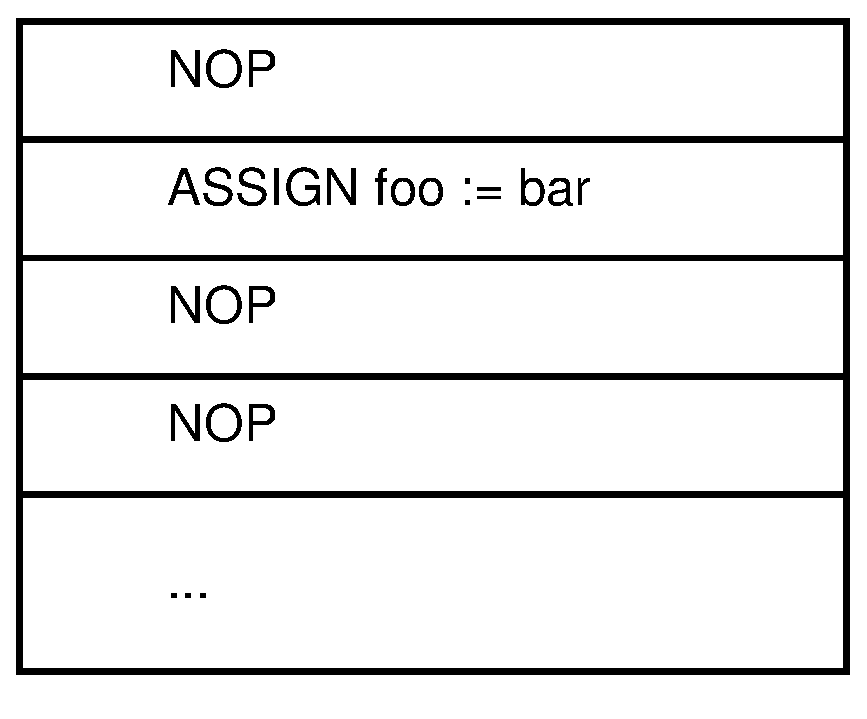
\includegraphics[scale=0.5]{figs/op-log.eps}
\caption{\label{fig:op-log}Operation Log}
\end{figure}

The operation log is a serial order of operations. It associates an `Operation ID' (OID)
with a particular operation. OIDs are integers and refer to indexes into the operation log. To
enter an operation into the log, the code picks the next highest instance ID that it has not seen
before and starts a new round of Paxos for that instance, trying to assert that
\verb$OID := <operation>$.

I tried a number of different techniques for retrying an insertion in the event that the OID was
associated with another operation. Initially I put the retry logic in the database. However it
became clear that it made more sense to delegate the responsibilty for retrying to Paxos.

This meant that at submit time the Database Controller could make no guarantee about the OID the
statement would have but did have the guarantee that once a statement was submitted to Paxos, it
would eventually be entered into the operation log.

As the database now only needed to pass the Paxos layer an operation the interface between the
database and Paxos was cleaner.  The database receives a callback when that statement was finally
entered into the transaction log with the OID it was entered as.\footnote{This would be the same
as the instance ID, as there is a one-to-one correspondence of OIDs $\leftrightarrow$ instance IDs).}

\subsection{Reads}

A distributed database has the concept of both \emph{fast reads} and \emph{slow reads}. A fast
read is a read that only examines the state of the database locally, without sending anything over
the network.  A slow read involves inserting an operation into the operation log in order to
ensure that the local copy of the database is up to date, then reading from that state.

A fast read has very low latency, as it does not need to send messages to any other nodes, but it
may return out of date data. A slow read forces the database to actually examine the current state
of the network by inserting an operation to ensure it has obtained all transactions issued
prior to the slow read.

In fact, I chose to use a \op{NOP} operation rather than a \op{READ} operation, although they
would semantically be the same (as other nodes do nothing on a \op{READ}), as I felt a \op{NOP}
better represented the operation being sent (do nothing).

\begin{figure}[htb]
\centering
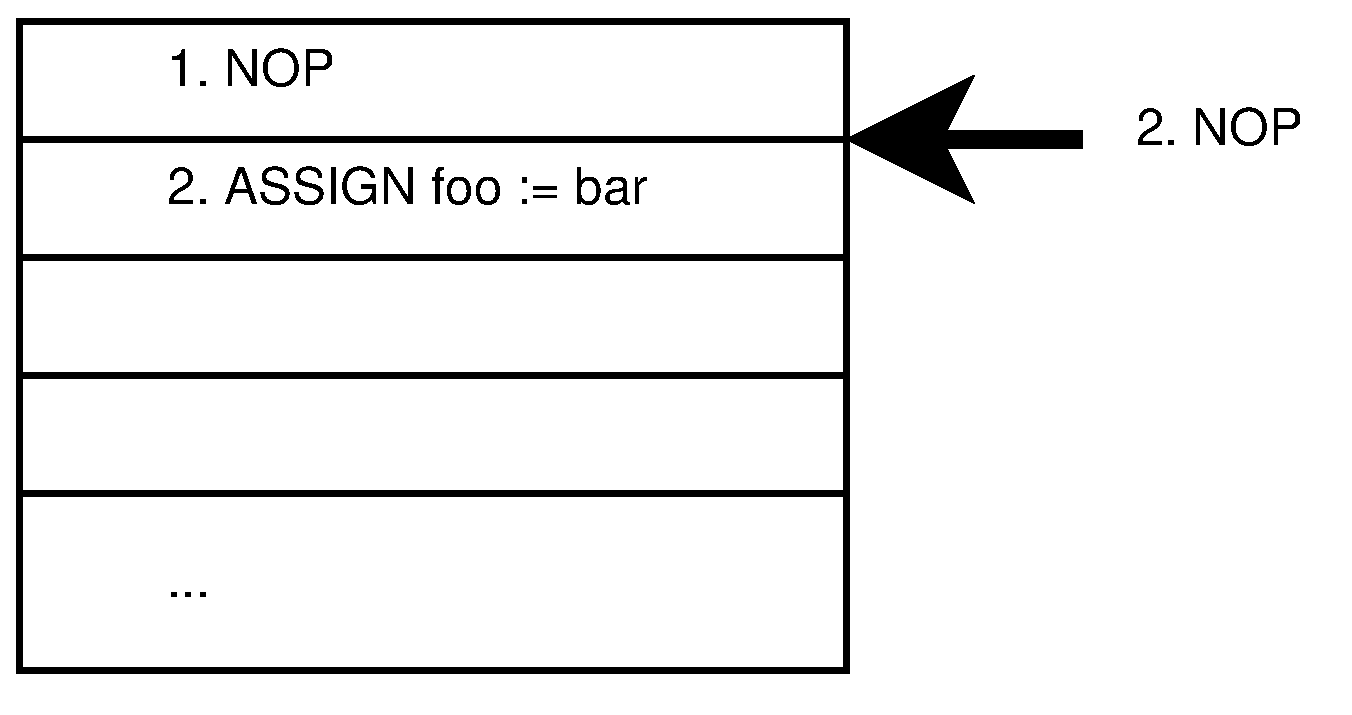
\includegraphics[scale=0.5]{figs/op-log-slow-read-1.eps}
\caption{\label{fig:op-log-slow-read-1}Performing a slow read}
\end{figure}

Figure~\ref{fig:op-log-slow-read-1} shows the situation as seen by a node $N$ at time $t_1$. It
has only received OID 1, as the \op{ASSIGN} in OID 2 has been learnt by the network but not by
$N$. In order to make sure $N$ is up to date with the network, it performs a slow read by trying
to insert a \op{NOP} at OID 2.

As the network has already learnt a value for OID 2, when $N$ tries to set it to a \op{NOP}, it
learns the value already decided by the network and retries with OID 3 instead. As no value has
been learnt for OID 3, $N$ succeeds in setting it to \op{NOP}.

\begin{figure}[htb]
\centering
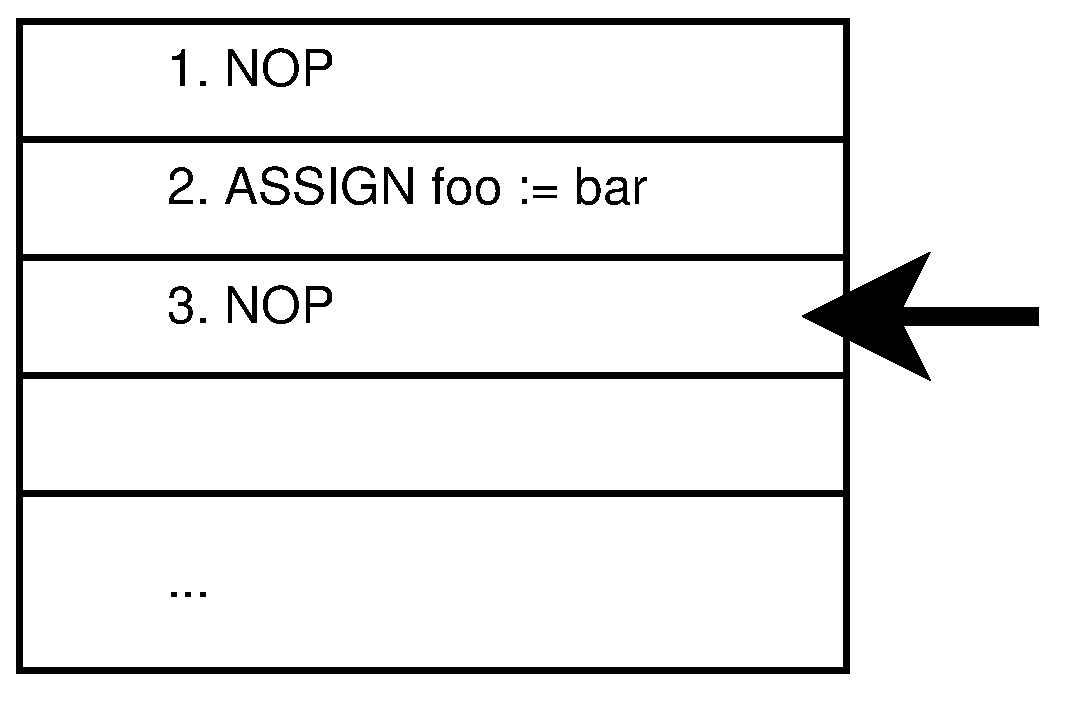
\includegraphics[scale=0.5]{figs/op-log-slow-read-2.eps}
\caption{\label{fig:op-log-slow-read-2}After a slow read}
\end{figure}

Figure~\ref{fig:op-log-slow-read-2} show the situation at time $t_2$ --- the \op{NOP} has been
inserted at OID 3 and from this $N$ knows that at $t_2$ the latest operation in the op-log the
slow read it just performed, i.e., it is up to date.

\subsection{Transactions}

\subsubsection{Global Lock}

\begin{figure}[htb]
\centering
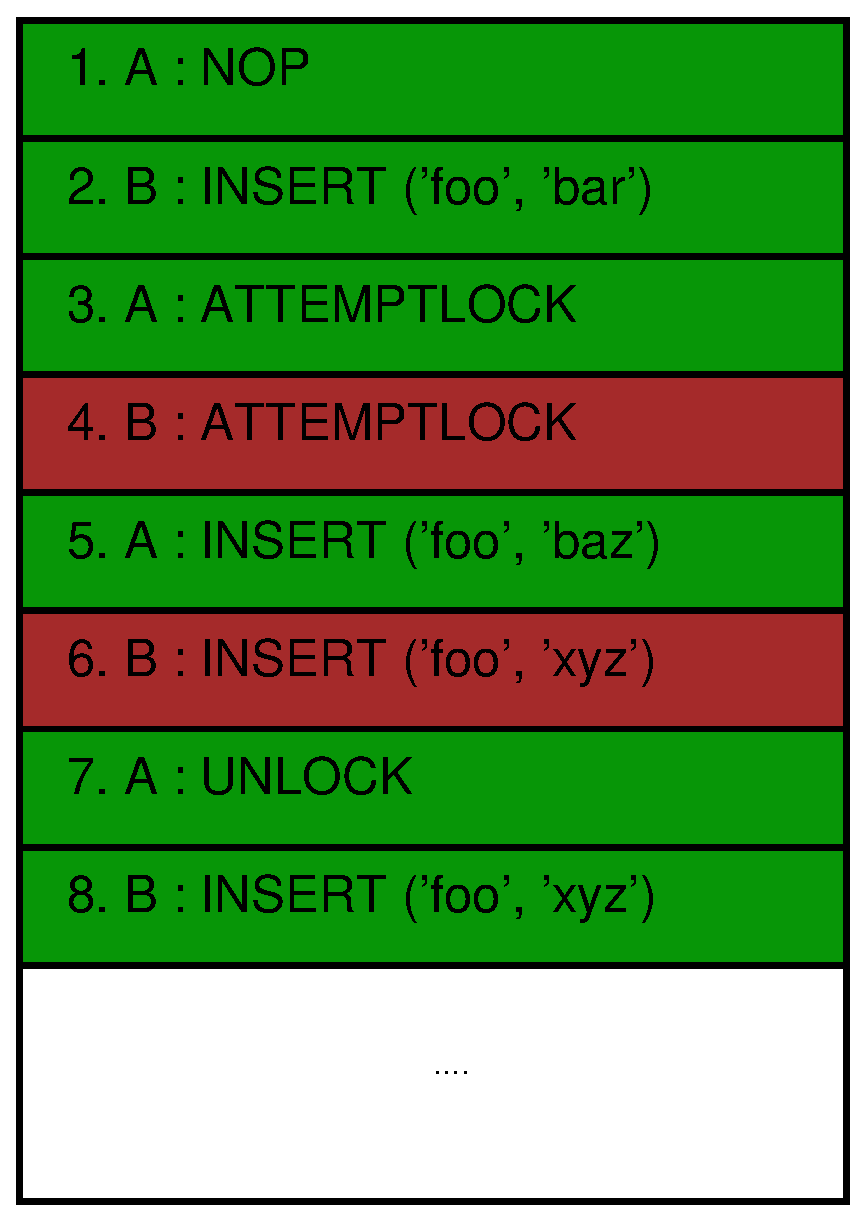
\includegraphics[scale=0.5]{figs/op-log-trylock.eps}
\caption{\label{fig:op-log-trylock}Transactions in the Operation Log}
\end{figure}

I implemented transactions with a simple global lock. This lock can only be held by one node at a
time and when a node holds it, only that node can perform operations on the database, providing
isolation for transactions.

In order to start a transaction, a node inserts the \op{ATTEMPTLOCK} operation. If, when the
operation is inserted, the number of preceeding \op{ATTEMPTLOCK}s is well-bracketed\footnote{There
is an equal number of lock takes and releases}, then the node was successful in taking the lock.
While a node holds the lock, no other node can perform an operation. Operations continue to be inserted
in the operation log but are not performed on the row store.

As an example, figure~\ref{fig:op-log-trylock} shows an operation log with two nodes
performing operations, nodes $A$ and $B$. In OIDs 1 and 2 neither node owns the global lock, so both
nodes are able to freely perform operations. Both try to take the lock and $A$ gets its operation
inserted first as OID 3, so now owns the lock. $B$'s operation is inserted as OID 4, so it has the
semantic meaning of a \op{NOP}. $A$ now performs an assignment under the lock (in reality this
would be a series of operations) as OID 5. As $A$ is the lock holder, the operation is performed.
$B$ tries to perform a different assignment, but as it does not hold the lock, the operation is
not performed. $A$ now releases the lock with an \op{UNLOCK} operation (OID 7). Finally, $B$
retries its assignment, which can finally be performed as no-one now holds the lock.

% \subsubsection{Two Phase Locking}
%
% I improved
%
% used two phase locking
% take locks in schema order to avoid deadlock and livelock
% restart transaction if locks taken out of order
%
% use strict 2PL to avoid cascading aborts
%
% potential further locking schemes?

\section{Database Implementation}

\subsection{SQL}

\subsubsection{Grammar}

I implemented SQL parsing using PyParsing, a python library that makes it easy to programmatically
construct simple grammars. Using this I constructed a grammar of the form:

\verb+SELECT (field1,field2,...) WHERE <where-clause>+ \\
\verb+INSERT (value1,value2,...)+ \\
\verb+DELETE WHERE <where-clause>+ \\
\verb+UPDATE SET k1=v1, k2=v2, ... WHERE <where-clause>+ \\

The grammar for the WHERE clause (marked as \verb+<where-clause>+ above) is more complex and
is presented below in production rules:
\begin{enumerate}
\item \verb+op -> == | != | < | > | <= | >=+
\item \verb+B  -> AND | OR+
\item \verb+T  -> f op f | ( C )+
\item \verb+C  -> T B T | T+
\item \verb+S  -> C EOL+
\end{enumerate}

In the above production rules \verb+f+ is either a fieldname, a string or an integer and \verb+EOL+
refers to the end of the string.

\subsubsection{Recursive Descent Parser}

\begin{figure}[Hhtb]
\centering
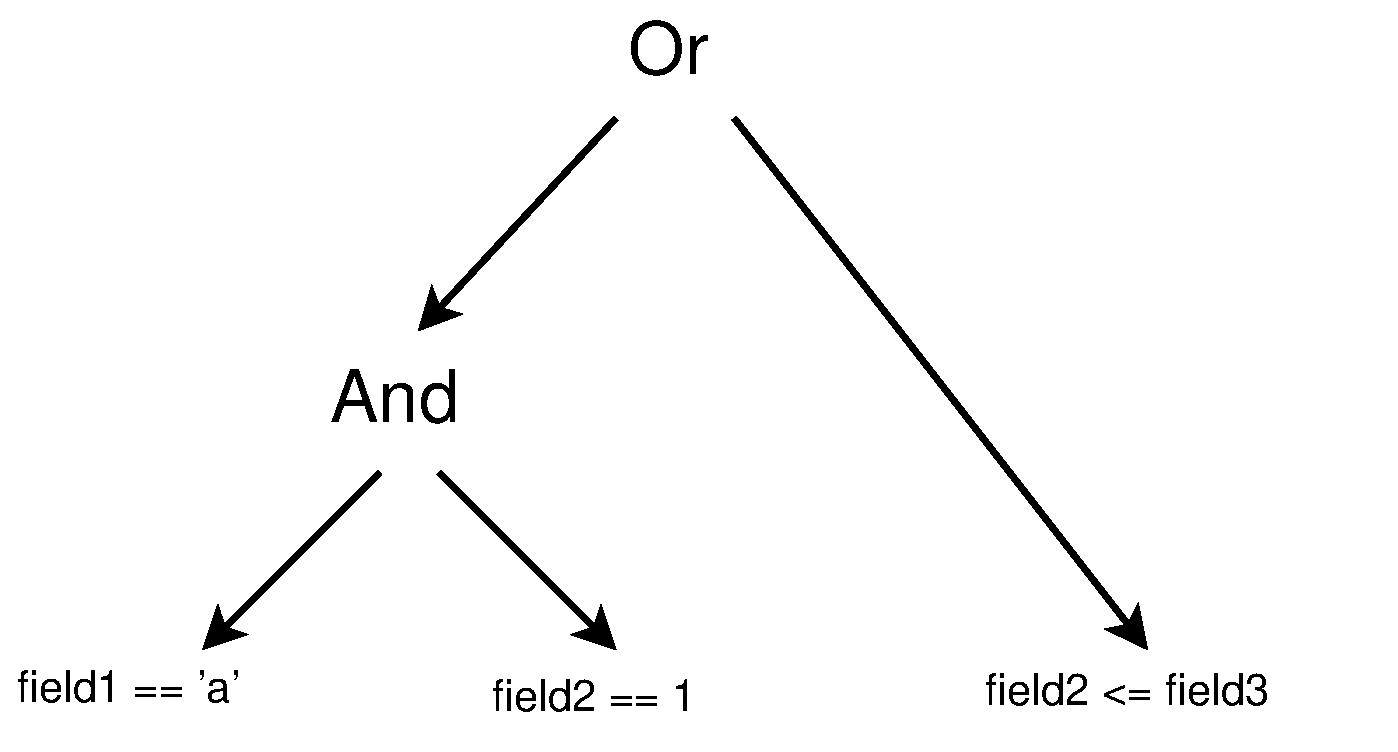
\includegraphics[scale=0.5]{figs/where-ast.eps}
\caption{\label{fig:where-ast}Example WHERE clause matching tree}
\end{figure}

For this grammar I then built a simple recursive descent parser to construct a boolean matching
tree. For example, the SQL fragment \verb+WHERE (field1 == 'a' AND field2 == 1) OR field2 <= field3+
would be parsed into the tree represented by figure~\ref{fig:where-ast}.

% How tools affected things
% Optimisation - `what it is'
% Talk about iterations
%
% SQL parser
% - what it supports
%
% -start up costs
%   - ping time etc
%   - inefficiencies
%   - cf. `supernodes' vs DHTs to organise nodes
%
% Talk about laptop breaking

% \section{Testing}
%
% I started off implementing unit tests for the
%
% \subsection{Commandline Tools}
%
% I implemented several commandline tools to interface with the main body of code. As I implemented
% Paxos

\cleardoublepage
\chapter{Evaluation}

After designing and implementing the system, I evaluated its performance against a number of
metrics. These were designed to measure how the system's performance differed with regard to
different parameters. The main parameters I varied were the number of nodes in the network and the
number of writers in the network. I also measured how the system performed in a situation with
limited bandwidth, and how the various improvements to the implementation that I made performed
against each other.

\section{Method}

There were a number of metrics I used to evaluate the system. The two main metrics were the
latency of an operation (how long it took to complete after being issued), and the throughput of
the system (how many operations could be completed in unit time). I also measured how the
bandwidth used varied in different situations.

\subsection{Simulation}

In order to evaluate the database the network was simulated on a single machine. This was necessary
for a number of reasons.

Firstly, it is impractical to create an actual network on a number of computers. Co-ordinating
tests between a large number of machines is difficult, and resources required were unavailable.

Also, as the number of nodes increases, it becomes increasingly difficult to get meaningful
results from nodes run on a physical network, due to other factors such as networking delay. It
also makes results inconsistent and difficult to reproduce on several runs. As my results are
dependent upon network characteristics, I wanted to control those characteristics.

Initially I spawned a separate instance of the test program for each node, but it became necessary
to run all nodes in the same script in order to control complex scenarios. I discuss the
limitations of this in the section below.

\subsubsection*{Assumptions}

For the simulation to be a valid measure of how the network responds, I made certain assumptions.
As a distributed application, I would expect my application to be mainly IO bound, rather than
being CPU bound. IO bound means that the application spends most of the time waiting for IO, in
this case network IO (sending and receiving messages), as opposed to CPU bound, which means the
application spends most of its time running on the CPU. The application must be IO bound for the
simulation to be valid -- if it is in fact CPU bound, running multiple nodes on the same machine
will lead to increased CPU load. This makes the simulation invalid, as the performance of the
simulated nodes will deviate from the performance of a real network due to the performance
depending on the CPU rather than the network.

However, as the network was simulated on one computer, this assumption did begin to break down as the
number of nodes increased. The problem was exacerbated because Python is limited to only using
one core without explicit parallelism, and Twisted's event loop ran for all the nodes in the
network. A potential fix would be to spawn different threads for each node and then join the
results when the simulation is done. In this way the simulation could utilise the full resources
of the simulating machine, instead of being artificially constrained by the resource limits of the
simulating machine. While this is possible in Twisted, it is not straightforward, and
unfortunately time constraints did not allow further exploration of this evaluation method.

\subsection{Gathering and Formatting Results}

I wrote a script that performed the actual simulation and output the data. The script took a
number of commandline parameters specifying the number of nodes in the network, the number of
writers, the number of operations to perform and the type of operations. It then constructed this
network and bootstrapped it. In order for the simulation to generate reliable results, the
operations could not immediately be run, the script had to wait for every node in the network
to be aware of every other node in the network. This start up time was not reflected in the
results. After the network bootstrapped, the required number of nodes were scheduled to write,
and the relevant metric in a CSV file was recorded in a CSV file.

5 measurements were taken for each point, the average and standard deviation were then caluated
and plotted by gnuplot. This was all co-ordinated from a Makefile, so that all graphs could
regenerated automatically. This automation meant I could review my data generation process
thoroughly to be sure it was valid, and be sure that I was handling all the data consistently.

\section{Contention}

I started off by measuring how the network responded to contention. This meant measuring how
the latency and throughput changed in response to the number of nodes in the network
which were writing. Obviously the higher the contention the longer it would take operations to
complete, but by graphing the results 

\subsection{Latency}

Latency was measured by scheduling an operation on each of the writing nodes concurrently and
recording the time each operation took to complete.

\begin{figure}[Hp]
\centering
%\lwincludegraphics[scale=2]{figs/lat_20.eps}
\subfigure[Latency for 5 Nodes]{
	\includegraphics[scale=0.75]{figs/lat_5.eps}
	\label{fig:lat-5}
}
\subfigure[Latency for 20 Nodes] {
	\includegraphics[scale=0.75]{figs/lat_20.eps}
	\label{fig:lat-20}
}
\subfigure[Latency vs Network Size] {
	\includegraphics[scale=0.75]{figs/lat_rev.eps}
	\label{fig:latency-rev}
}
\end{figure}

\paragraph{5 Nodes}

Firstly I measured the contention in a network with 5 nodes. Figure~\ref{fig:lat-5} shows how the
average latency of an operation was affected by the the number of writers in the system. Plotted
on the graph are three different types of network operations: the latency of a pure Paxos
operation, the latency of a single database operation and the latency of a database transaction.
The first two lines are very close, this is expected as a database operation is simply a specific
Paxos operation. The minor difference is due to the database processing overhead. As mentioned in
the Method section, this overhead is expected to be minor, as the application is mainly IO bound
rather than CPU bound. However, a small amount of added CPU latency is reasonable.  The latency of
transactions is significantly more than that of database operations. This is also expected as
executing a transaction involves waiting on several Paxos operations to be executed before it is
committed.

A common trend in the graph is that the latency of committing an operation to the
network increases linearly with the number of writers in the network with a strong
correlation.

\paragraph{20 Nodes}

I repeated the simulation with a network of 20 nodes. Figure~\ref{fig:lat-20} shows
the latency of the network continues to increase linearly with the number of concurrent writers in
the system.

\paragraph{Network Size}

I also measured how the network response time is affected by the number of nodes in the network.
Using only a single writer, I measured the latency for networks of varying sizes. This is
displayed in figure~\ref{fig:latency-rev}.

\subsection{Throughput}

\begin{figure}[Hp]
\centering
\subfigure[Throughput for 5 Nodes]{
	\includegraphics[scale=0.75]{figs/thru_5.eps}
	\label{fig:thruput-5}
}
\subfigure[Throughput for 20 Nodes]{
	\includegraphics[scale=0.75]{figs/thru_20.eps}
	\label{fig:thruput-20}
}
\subfigure[Throughput vs Network size]{
	\includegraphics[scale=0.75]{figs/thru_rev.eps}
	\label{fig:thruput-rev}
}
\end{figure}

Next I measured the throughput of the network. This is the number of operations per second that
can be processed by the network. Again I plotted three lines for each graph --- paxos throughput,
database operation throughput and database transaction throughput.

I measured the throughput by measuring how long it took to commit 5 operations to the network with
a given number of writers. I did this 5 times for each writer and then took the average and
standard deviation of each point. I then plotted $\frac{5}{x}$ for each point as the average throughput in
\emph{operation seconds\superscript{-1}}.

\paragraph{5 Nodes}

Again I initially did this for a network of 5 nodes. The results of this are in
figure~\ref{fig:thruput-5}, which shows that the throughput of the network decreases with
$\frac{1}{w}$, where $w$ is the number of concurrent writers in the system. Again the performance of
Paxos and database operations is similar, with very similar throughputs. However there is still a
big overhead to using transactions, as evidenced from the substantially reduced throughput,
reduced by nearly a factor of 5.

\paragraph{20 Nodes}

Figure~\ref{fig:thruput-20} shows the throughput of the network decreases exponentially with the
number of concurrent writers in the system. Also while there is little overhead from using the
database layer over the top of Paxos, there is substantial overhead performing multiple
transactions.

\subsection{NACK improvements}

\begin{figure}[Hhtb]
\centering
\lwincludegraphics[scale=2]{figs/lat_nack.eps}
\caption{\label{fig:nack}NACK improvement}
\end{figure}

Figure~\ref{fig:nack} shows how the different NACK implementations compare against each other in
terms of latency. The increase in latency is linear with all implementations, but there is a clear
improvement from using NACKs. As contention increases the number of Proposers competing for
Acceptors to accept their proposals increases, so the latency would be expected to increase.
Interestingly there is not a clear different between NACK `version 1' and not using NACKs. This
may be due to the `ping pong' effect mentioned in the Implementation chapter. Although NACKs would
reduce the amount of timeouts occuring, it may increase the contention between Proposers and the
number of messages sent, without offering an increase in latency.

\subsection{Start up costs}

\begin{figure}[Hhtb]
\centering
\lwincludegraphics[scale=2]{figs/start.eps}
\caption{\label{fig:start}Start}
\end{figure}

As the size of the network increases the cost of bootstrapping the network becomes prohibitively
expensive. Figure~\ref{fig:start} shows the effect of using a master node to co-ordinate the
network instead of the initial peer-to-peer bootstrap design. The peer-to-peer design fits an
$N^2$ curve as the number of nodes in the network increases, as expected, as every node messages
every other node. In the centralised design, not only is the amount of bandwidth used at the start
significantly decreased, but the increase as the number of nodes rises in linear, rather than
$N^2$.

\subsection{Node Churn}

\begin{figure}[Hhtb]
\centering
\subfigure[Latency vs Churn]{
	\includegraphics[scale=0.75]{figs/churn_lat.eps}
	\label{fig:churn-lat}
}
\subfigure[Throughput vs Churn]{
	\includegraphics[scale=0.75]{figs/churn_thru.eps}
	\label{fig:churn-thru}
}
\end{figure}

Paxos is designed to remain fully functional as long as a majority of nodes remain in the network.
I measured how the network responds to nodes leaving and joining the network.
Figure~\ref{fig:churn-lat} shows how the latency of an operation is affected by nodes leaving and
joining a network of 20 nodes. The churn has no effect until a majority of nodes start leaving the
network, when the performance suddenly drops off.

This can also be seen in figure~\ref{fig:churn-thru}, which shows how the throughput of the
network is affected by churn, again in a network of 20 nodes. The result is similar -- the churn
has no effect until a majority of nodes are affected, at which point the network is unable to make
any progress.

\section{Limitations}

The main limitation of the system is its speed. In particular, transactions, a core component of
any database, have a large cost.

Another limitation is the lack of stable storage support in the database. Although it supports
durability in that, if a node leaves, and then returns, the operation will persist in the network
and if that node rejoins, then it will see the transaction again, if a majority of nodes leave and
rejoin, the database will lose its transactions as it has no stable storage and a majority of
nodes have failed. However if the nodes leave slowly enough for the network quorum to adjust it
will be fine.

Another drawback is that the network struggles to function as its size increases - the way I have
implemented Paxos is easy to debug but is very verbose. Using a more efficient variant such as
MultiPaxos would decrease the bandwidth requirements of the system. Alternatively using a variant
such as FastPaxos would decrease the latency.

Although I show an improvement to the startup cost of bootstrapping the network, my improvement
only centralises the bootstrapping, losing all the advantages of using a distributed network. A
complete solution would be to use a DHT or super-node hierarchy.

Due to time constraints I did not have time to implement all the SQL syntax that my requirements
indicated. However this is not a significant concern as it is relatively easy to add new syntax and
operations to the database.

\section{Changes with hindsight}

If I was to do the project again, there are several potential changes that I could make.

% Although my project is built in an asynchronous manner and used Twisted, with the knowledge I have
% gained from implementing it, a potential change would be to write it in a synchronous style.
% Decoupling from Twisted may allow further opportunities for optimisation and
% These mainly
% are design choices more than anything else. One big design choice I made was to use an
% asynchronous programming paradigm. I chose this because I thought it would make the project
% simpler and quicker to write, by leveraging Twisted's network stack. However I didn't allow for
% the difficulty of understanding and designing Paxos, or a database, or Paxos and a database under
% a new programming paradigm.

One design choice I made was to start with a key/value database prototype and later
refactor it into a row based database. I then added an SQL interface and layered transactions on
top. This was a reasonable choice, as I started small and then worked bigger. However if I was to
do the project again using my knowledge from my first implementation, I would be able to
design the system as row-based from the start.

% Also, in my project the SQL interface is built as a layer on top of the database. This makes it
% easy to extendThe SQL interface should have been more
% tightly integrated rather than less tightly, and transactions should have been the core aspect of
% my system, rather than a layering of operations. However it is difficult to predict how the
% project would have turned out with this plan, it is not necessarily as easy to implement as it
% sounds and I believe my choices were very reasonable at the time.

% Another possibility is that I should have started with smaller prototypes of the complete system,
% rather than prototypes of both of them that were then joined. A disadvantage of my approach was
% that as my understanding of how the design would work progressed, the API interface between the
% two components changed significantly and repeated. This led to problems with testing, and with
% having to rewrite various user interfaces repeatedly. An alternative approach could have been to
% use an agile programming strategy, rather than an iterative one. A quote that summarises my
% experience with my project is by Fred Brooks: `plan to throw one away; you will, anyhow'.

% \subsection*{Twisted}
%
% In retrospect, if I was to do the project again I would probably not use Twisted. Twisted provided
% me with a powerful framework for building an asynchronous network application, but it had
% disadvantages as well as advantages, which I will briefly outline.
%
% I had to learn a lot for this project. I had to learn and understand how how Paxos works and
% design a protocol that implements it. I also had to learn and understand the basics of building a
% database, and on top of that - a distributed database. Twisted has a high learning curve, and I
% ended up investing a lot of time understanding how to work with Twisted and in some cases working
% against it. I spent lots of time interfacing with it, some of which was unnecessary.
%
% It is difficult to know how much networking code Twisted saved me writing, however
% the message requirements of paxos are quite simple, and I think that with a few days work making
% some helper network classes much of the complexity of using and interfacing with Twisted could
% have been avoided. Certainly there are cases when debugging would have been easier, and I feel my
% project would have been less `heavy-weight', particularly when it came to unit tests, another
% problem I will discuss later.
%
% As I worked through several prototype versions, Twisted became cumbersome to use. I had to keep
% learning new parts of it, which was frustrating to have to keep delving into the innards of it,
% particularly as I started to feel that it hadn't helped me as much as I had anticipated.
%
% Using the asynchronous paradigm initially helped me reason about Paxos and how I would design my
% system, however later on I felt the asynchronous model was unnecessary, and Twisted became
% superfluous. Certainly my project would have been very different without the decision to use it.

\subsection*{Testing}

Unit tests became a problem as I progressed through the project. They became a hindrance, as I
was refactoring my code base often, they were not that effective. Test Driven Development may have
been a better choice, as I wrote my unit tests after I had written the code, I would often write
the code, write the tests, it would all work. Then I would refactor the code, rewrite the tests ---
every refactoring would invalidate large numbers of tests. This was also due to how tightly
coupled my code was with Twisted. This is another reason I would reconsider my decision to use
Twisted if I were to redo the project.

% \section{Summary}

% In summary, my project had clear successes but also some clear drawbacks. I effectively
% implemented Paxos, and built an ACID distributed database on top, with support for transactions. I
% made some improvements to my design, but ultimately there are still many more clear avenues for
% improvement. The project suffers from inefficiency, and is slow, but is an effective prototype
% that gives valuable insight into the performance ramifications of different design decisions of a
% distributed database. My project was limited not just by the limited amount of time I had, but
% also by my lack of expertise in the area, and I have gained valuable insights into my decisions
% and how I would improve the project if I were to implement it again.


\cleardoublepage
\chapter{Conclusion}

\section{Comparison with Requirements}

The requirements are a formal list of elements of the project to be
considered in evaluating its success. I will outline them here and discuss how each was realised,
and to what extent.

\subsection{Paxos}

The project successfully meets the requirements of being able to form a running network which can
achieve consensus. It can perform dynamic leader election through the Paxos network, and
supports nodes joining and leaving arbitrarily. This area of the success criteria was met fully.

\subsection{ACID}

The ACID success criterion was to support all ACID properties - Atomic, Consistent, Isolated and
Durable. The project supports all of them as long as the network persists - there is no support
for stable storage.

\subsection{SQL}

The success criterion for SQL was designed to reduce the scope of SQL in order to allow me to
focus on the design of the Paxos protocol and the database. It was reduced to a single table with
a static name, SELECT and INSERT statements, including a WHERE clause.

\section{Further Work}

There are multiple opportunities that could be investigated given more time that would allow for
the project to be improved and extended.

\paragraph{Transactions}

There are several different locking schemes that could be used Optimistic Concurrency Control
(OCC) being one of particular interest, as it is much more effective in a network with low
contention.

\paragraph{Durability}

Supporting stable storage as a means of ensuring durability through the use of write-ahead logs
(WAL)\cite{burrows06} and/or shadow paging\cite{hitz94}.

\paragraph{Network Hierarchy}

Other mature techniques used to manage large networks efficiently could be investigated, such as
using `supernodes' or Distributed Hashing Tables.

\paragraph{MultiPaxos}

Using the more efficient MultiPaxos and FastPaxos variants would allow an
increase in efficiency both in terms of network throughput and latency, and also in terms of
bandwidth.

\paragraph{Security}

One area of Computer Science that I constantly encountered during this project was security.
Although I decided it was beyond the scope of my project, given more time it would have been
valuable to investigate the security implications of many of my design decisions and build more
security into my design, as well as considering implementing Byzantine Paxos, which can tolerate
rogue and faulty nodes in the network.

\cleardoublepage

%%%%%%%%%%%%%%%%%%%%%%%%%%%%%%%%%%%%%%%%%%%%%%%%%%%%%%%%%%%%%%%%%%%%%
% the bibliography

\addcontentsline{toc}{chapter}{Bibliography}
\bibliography{refs}
\cleardoublepage

%%%%%%%%%%%%%%%%%%%%%%%%%%%%%%%%%%%%%%%%%%%%%%%%%%%%%%%%%%%%%%%%%%%%%
% the appendices
\appendix

\chapter{Paxos Pseudocode}

\section{Proposer}

\subsection{Phase 1}

\begin{algorithm}[H]
 %\SetAlgoLined
 \For{each node n in the network}{
   Message(n, \msg{Propose(p)})
 }
 \caption{Phase 1 Proposer Algorithm}
\end{algorithm}

\subsection{Phase 2}

\begin{algorithm}[H]
 %\SetAlgoLined
 % \KwData{this text}
 % \KwResult{how to write algorithm with \LaTeX2e }
 Quorum.add(msg.uid) \\
~\\
 \If{msg.PrevPropNum exists}{
  \If{msg.PrevPropNum $>$ PrevPropNum}{
    PrevPropNum := msg.PrevPropNum
    PrevPropValue := msg.PrevPropValue
  }
 }
 \caption{Promise Message Handler Algorithm}
\end{algorithm}

\section{Acceptor}

\subsection{Phase 1}

\begin{algorithm}[H]
 %\SetAlgoLined
 \If{msg.PropNum $<$ PreparePropNum}{
    writeMessage(msg.uid, \msg{Promise}(msg.PropNum, CurPropNum, CurPropValue)) \\
    PreparePropNum := msg.PropNum
 }
 \caption{\msg{Prepare} Message Handler Algorithm}
\end{algorithm}

\subsection{Phase 2}

\begin{algorithm}[H]
 %\SetAlgoLined
 \If{msg.PropNum $\ge$ PreparePropNum}{
   CurPropNum := msg.PropNum \\
   CurPropValue := msg.PropValue \\
   writeAll(\msg{AcceptNotify}(PropNum, PropValue))
   }
   \caption{\msg{AcceptRequest} Message Handler Algorithm}
\end{algorithm}

\section{Learner}

\begin{algorithm}[H]
 %\SetAlgoLined
 accepted[PropNum].add(msg.uid) \\
 \If{len(s) $\ge$ QuorumSize}{
  status = "completed" \\
  value = msg.PropValue \\
  callback.fire(instance)
 }
 \caption{\msg{AcceptNotify} Message Handler}
\end{algorithm}

\chapter{Code Sample}

\begin{lstlisting}
def datagramReceived(self, msg, host):
    """Called when a message is received by a specific agent.

    """
    self._msgs.append((msg, host))
    try:
        m = parse_message(msg)
        # If we haven't heard this host before, add them to the record
        if m['uid'] not in self.hosts and m['uid'] != self.uid:
            self.addHost(m['uid'], host)
        t = m['msg_type']
        dbprint("Got %s message from %s\n%s\n" % (m['msg_type'], host, m), level=1)
        if m['instance_id'] is not None:
            i = m['instance_id']
            if i not in self.instances:
                if i >= self.current_instance_number:
                    self.current_instance_number = i+1
                self.instances[i] = self.create_instance(i)
            else:
                assert i < self.current_instance_number, \
                "known but oddly large instance number %s (%s)" % (i, self.current_instance_number)
            instance = self.instances[i]
            if instance['status'] == 'completed':
                dbprint("dropping msg as instance %s is already completed" % i, level=2)
                return
        else:
            instance = None
        method = getattr(self, "recv_%s" % t)
        method(m, instance)
    except (InvalidMessageException, KeyError), e:
        dbprint("%s received invalid message %s (%s)" % (self, msg, e), level=4)
        raise
\end{lstlisting}

\chapter{Project Proposal}

\vfil

\centerline{\Large Computer Science Project Proposal}
\vspace{0.4in}
\centerline{\Large PDB: A Distributed Database Based on Paxos}
\vspace{0.4in}
\centerline{\large Charlie Shepherd, Churchill College}
\vspace{0.3in}
\centerline{\large Originator: Charlie Shepherd}
\vspace{0.3in}
\centerline{\large 18$^{th}$ October 2012}

\vfil


\noindent
{\bf Project Supervisor:} Stephen Cross
\vspace{0.2in}

\noindent
{\bf Director of Studies:} Dr John Fawcett
\vspace{0.2in}
\noindent

\noindent
{\bf Project Overseers:} Dr~A.~Madhavapeddy \& Dr~M.~Kuhn


% Main document

\section*{Introduction, The Problem To Be Addressed}

{\em Paxos} is a protocol for achieving distributed consensus, developed by Leslie Lamport in 1991.

The motivation for Paxos as a protocol is that it is capable of handling failures that other
consensus protocols cannot. {\em Two Phase Commit} (2PC) and {\em Three Phase Commit} (3PC) are two common
protocols that can be used to ensure atomic commits in a distributed system.

2PC works by having a co-ordinator node contact every node and send a proposal message. Each node
must then either respond with a commit or abort message. However, 2PC suffers from several
problems, mainly that it is a blocking protocol. This means that if the co-ordinator fails, and
then a node subsequently fails, the network will deadlock, as 2PC is not able to recover from that
failure situation.

3PC is an extension to 2PC which endeavours to fix this limitation, at the expense of greater
latency, by adding a third roundtrip to confirm the commit to all nodes. This means that the
protocol is asynchronous, and that node failures cannot block the protocol or cause it to fail.
However, it still has its own limitations, in particular, in the event of a network partition. If
the network is partitioned so that in one partition all nodes vote ``commit'' and in the other all
nodes vote ``abort'' both partitions will initiate recovery, and when the network merges again the
system will be in an inconsistent state. This is the limitation that Paxos was intended to solve.

My project will be to design and implement a distributed database, built on the Paxos protocol.


\section*{Starting Point}

My starting point will be to study the Paxos protocol, as well as research distributed databases.
From there I will develop a library implementing Paxos, along with unit tests. I will then design
and implement a distributed database on the Paxos library. The challenge will be to implement a
complex distributed protocol and then utilise it for a database, as these are both areas I have
little experience of.

\section*{Resources Required}

I will mainly do my project on a virtual machine which is running on my own personal laptop.
The source code will be committed to a Git repository, which will be pushed to Bitbucket and my
own personal host. The virtual machine contents will be backed up on an external HDD for quick
recovery, although the git repository will be adequate for restoring my project if the system I am
developing it on fails.
I require no other special resources.

\section*{Work to be done}

The project breaks down into the following sub-projects:

\begin{enumerate}

\item A study of distributed algorithms and the Paxos protocol

\item A study of distributed databases

\item Implementing the Paxos protocol

\item Designing the distributed database

\item Implementing the distributed database

\item Evaluating the performance of the database

\end{enumerate}

\section*{Success Criteria for the Main Result}

In order for the project to be a success, the following must be true:

\begin{enumerate}

\item The project must correctly implement the Paxos protocol.
	The library must be capable of forming a running network,
	in particular dynamic leader election,
	as well as achieving consensus on a key/value store across the network.

\item The database must implement a subset of SQL, specifically:
\begin{enumerate}
\item A single table with a static name
\item SELECT/INSERT
\item WHERE
\item GROUP BY
\item ORDER BY
\item Aggregation
\end{enumerate}

\item The database must have all ACID properties, that is:
\begin{enumerate}
\item Atomic
\item Consistent
\item Isolated
\item Durable
\end{enumerate}

\end{enumerate}

\section*{Evaluation Topics}

There are several potential evaluation metrics for the project.

One major metric is transaction latency - the time for a transaction to be committed to the system. This
can be evaluated in a number of difference circumstances, including simulated node failure, leader
failure and network partition, and the results analysed to see how the system handles performance
under failure compared to normal conditions.

Another key metric is transaction throughput - the maximum number of transactions committed to the
network over a specified period of time. Again there are a number of different situations
throughput can be measured in, including load from one source, load from multiple sources and
load under failure.

I will also investigate the advantages of a distributed database over a normal single-server
database, particularly in terms of scalability. I will also consider how performance is affected
by the ratio of writing clients to reading clients.

\section*{Possible Extensions}

A clear possible extension is to investigate various different modifications to Paxos in order
to try to optimise the database for certain performance characteristics
(e.g. fast reads, but slow writes),
and to assess the usefulness and efficiency of these modifications.

Another possible extension is to investigate how the database performs when various ACID
properties are relaxed, and to measure and analyse how the performance gains compare with the
tradeoffs made.


\section*{Timetable: Workplan and Milestones to be achieved.}

\setlength\parindent{0pt}
\parskip = \baselineskip

Planned starting date is 19/10/2011.

\subsection*{Michaelmas Term}

{\bf 19/10/2012-01/11/2012} Research distributed algorithms and the Paxos protocol; design the
protocol implementation and library layout.

Milestone: A write up of the Paxos algorithm and a design document of the implementation.

{\bf 02/11/2012-15/11/2012} Begin the protocol implementation.

Milestone: Basic Paxos implementation.

{\bf 16/11/2012-29/11/2012} Finish implementation of Paxos library.

Milestone: Paxos implementation that can coordinate distributed leader election and achieve
consensus, including unit tests.

\subsection*{Christmas Vacation}

{\bf 30/11/2012-13/12/2012} Research distributed databases and design the database implementation.

Milestone: A write up of research on distributed databases and a design document for the database.

{\bf 14/12/2012-27/12/2012} Slack time/Revision/Holiday break.

{\bf 28/12/2012-10/01/2013} Prepare for progress report, start database implementation.

Milestone: Draft progress report, initial database implementation.

\subsection*{Lent Term}
{\bf 11/01/2013-24/01/2013} Write progress report, finish database implementation.

Milestone: Finished Progress report, fully functional database implementation.
Deadlines: Progress report deadline - 01/02/2013.

{\bf 25/01/2013-07/02/2013} Perform initial performance analysis on transaction, including
transaction latency and transaction throughput.

Milestone: Initial analysis data.

{\bf 08/02/2013-21/02/2013} Perform detailed performance analysis comparing distributed and
centralised servers, and on failing and partitioned networks.

Milestone: Analysis data on server models and on performance during failure.

{\bf 22/02/2013-07/03/2013} Investigate improvements to the protocol/implementation and their effect on
performance metrics.

Milestone: Improvements to protocol/implementation and revised performance data.

{\bf 08/03/2013-21/03/2013} Start dissertation.

Milestone: Draft Introduction and Preparation sections complete.

\subsection*{Easter Vacation}

{\bf 22/03/2013-04/04/2013} Finish writing up dissertation.

Milestone: Draft Implementation, Evaluation and Conclusion sections complete.

{\bf 05/04/2013-18/04/2013} Proof reading and then an early submission so as to concentrate on
examination revision.

Milestone: Finished dissertation.

\subsection*{Easter Term}
{\bf 19/04/2013-02/05/2013} Slack time/Revision/Holiday break.

{\bf 03/05/2013-16/05/2013} Slack time/Revision/Holiday break.

Deadlines: Official dissertation submission deadline - 17/05/2013.


\end{document}
